% !TeX root = ../ecuaciones-diferenciales.tex

\chapter{Introducci\'{o}n a las ecuaciones diferenciales}

\section{Idea intuitiva}
\begin{dfn}[Ecuación diferencial de primer orden]
	Sea $\mbf{y} = f(x)$, una \textbf{ecuación diferencial de primer orden} es una ecuación de la forma: $\mbf{y'}=F(x,\mathbf{y})$.\\
    Sea $g(x)$ una función de x, diremos que es solución cuando la ecuación diferencial se cumpla para $\mbf{y} = g(x)$.
\end{dfn}

Veamos unos ejemplos típicos.

\begin{eg}
    Consideramos $\P \equiv x'(t) = 2x(t)$ (o alternativamente $\mbf{x}' = 2\mbf{x}$)\\
    Vemos que es una ecuación diferencial de primer orden ya que sigue la definición anterior. Es sencillo ver que $F(t,\mbf{x}) = 2\mbf{x} = 2x(t)$. Queremos hallar que funciones resuelven $P$\\
    Además, observamos que si $x(t) = e^{2t}$, entonces $x'(t) = 2e^{2t} = 2x(t)$ y por tanto $x(t) = e^{2t}$ es una solución de $P$.\\Si pensamos con más cuidado también observamos que $x(t) = 7e^{2t}$ también satisface $P$.\\
    Nos interesaría entonces hallar una \textbf{solución general}, que con una sola ecuación englobe todas las soluciones. Aunque de momento no podemos justificarlo, si tomamos $x(t) = ae^{2t} \mid a \in \R$ entonces se cumple que $x'(t) = 2ae^{2t} = 2x(t)$ y por tanto es la solución general de $P$.
\end{eg}

Del ejemplo anterior surgen problemas llamados \textit{problema de valor inicial}, donde hallando la solución general y sabiendo la imagen de un punto $t_0$ por medio de $x(t)$ podemos determinar el parámetro y encontrar una solución explícitamente. Como continuación al ejemplo anterior consideremos el sistema:
$$
    \begin{cases}
        x'(t) = 2x(t) \\ x(0) = 8
    \end{cases}
$$
Para resolverlo, hallamos la solución general $x(t) = ae^{2t}$ y sustituimos la segunda ecuación. $x(0) = ae^{0} = 8 \implies a = 8$.

\begin{eg}
    Consideramos $\P \equiv x'(t) = 3(x(t))^{\sfrac{2}{3}}.$, queremos hallar \textit{la} solución para $x(0)=0$.\\
    Empezamos hallando soluciones a la ecuación, en este caso $x(t) = t^3$ y $x(t) = 0$ resuelven la ecuación. Nuestro sistema sería:
    $$
        \begin{cases}
            x'(t) = 3(x(t))^{\sfrac{2}{3}} \\ x(0) = 0
        \end{cases}
    $$
    Sin embargo, tanto $x(t) = t^3 \mid t = 0$ como $x(t) = 0$ resuelven $P$. No podemos hablar de \textit{la} solución puesto que hay dos.
\end{eg}

En los dos ejemplos anteriores tenemos una ecuación diferencial de la forma $\mbf{x'} = F(t, \mbf{x})$, $f(\mbf{x}) = 2\mbf{x}$ y $f(\mbf{x}) = 3\mbf{x}^{\sfrac{2}{3}}$ respectivamente. Sin embargo, en la segunda tenemos dos soluciones para $x(0) = 0$. Al observar las gráficas de las dos funciones se ve la razón a simple vista, la segunda no es derivable en $0$.
\begin{center}
    \begin{tikzpicture}
        \begin{axis}[domain=-5:5,samples=150,
        restrict y to domain=-10:10,
        xtick=\empty,ytick=\empty,
        %extra x ticks={0.8,1.4}, linea vertical
        %extra y ticks=3.333333,extra y tick labels={$\frac{10}{3}$}, linea horizontal
        grid=both,axis lines=middle
        ]
            \addplot+[no marks, thick] ({x},{2*x}) node[pos=0.3, below, sloped] {$f(x)=2x$};
            \addplot+[no marks, black, thick,samples=400] ({x},{3*x^(2/3)}) node[near end, below, sloped] {$f(x)=3x^{\sfrac{2}{3}}$};
            \addplot+[no marks, black, thick,samples=400] ({-x},{3*x^(2/3)});
        \end{axis}
    \end{tikzpicture}
\end{center}

\begin{eg}[Crecimiento de una población]
    Consideramos $\P \equiv \mbf{x'} = \lambda \mbf{x}$. ($\lambda$ típicamente es natalidad o mortalidad).\\
    Sabiendo que modela el crecimiento de una población en función del tiempo, podemos aproximar (veremos por qué más adelante)
    $\frac{\Delta x}{\Delta t} \sim \dd{x}{t} = \mbf{x'}$. Por tanto (como $\lamda$ es una tasa, se entiende que el tiempo tiende a 0 para hallarla):
    $$ \frac{\Delta x}{\Delta t}\sim \dd{x}{t} = \lambda \cdot \mbf{x} \implies \lambda = \lim_{t \to 0} \frac{\mbf{x'}}{\mbf{x}}$$.
\end{eg}

El crecimiento de una población de organismos lo suficientemente grandes no se ve representada por la ecuación anterior debido a la limitación de recursos. Interesaría por tanto modelizar la ecuación teniendo esto en cuenta. Para ello utilizaremos el parámetro $L$ como el límite al que tendería la población con los recursos existentes.

\begin{eg}[Crecimiento de una población con limitación de recursos]
    Consideramos $\P \equiv \mbf{x'} = a(1-\frac{\mbf{x}}{L})\mbf{x}$ con $a > 0$. De esta forma cuando $\mbf{x} << L$ o $\mbf{x} >> L$ , tenemos prácticamente la ecuación del ejemplo anterior. Si $\mbf{x} \sim L$ entonces la población apenas crece/decrece. Para encontrar soluciones a esta ecuación no hace falta resoverla, basta graficarla. Partimos de $\mbf{x'} = f(t, \mbf{x}) = a (1 - \frac{\mbf{x}}{L})\mbf{x}$.
    \\
    \begin{center}
        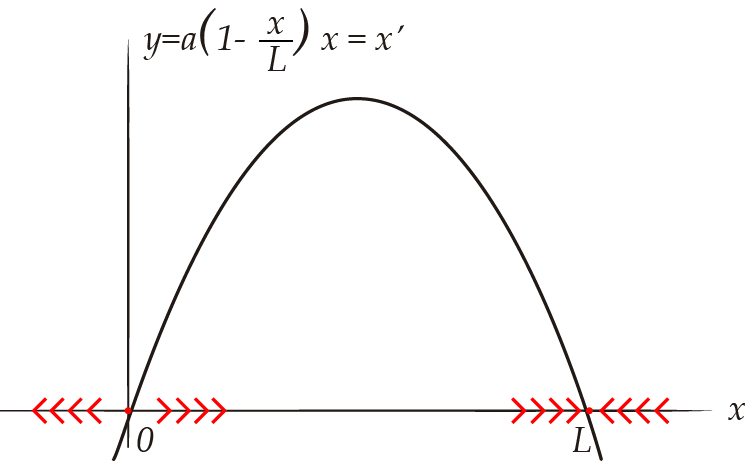
\includegraphics{1-limiterecursos.png}\label{img:1-limiterecursos}
    \end{center}
    Es fácil ver que $\mbf{x'}$ es una parábola, que corta al eje X en $0$ y $L$. Además, se indica con (>>) la dirección en la que se mueve $x(t)$ conforme avanza $t$. Tanto $0$ como $L$ son puntos de equilibrio, repulsor (inestable) y atractor (estable) respectivamente.
\end{eg}
\break

\begin{wrapfigure}{r}{0.5\textwidth}
  \begin{center}
    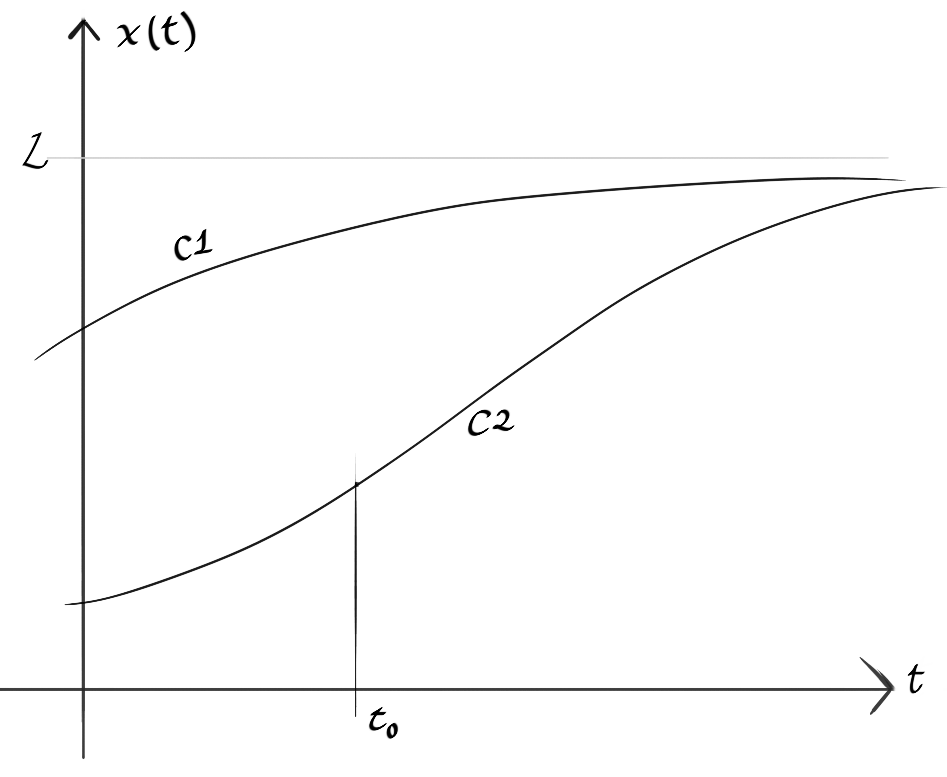
\includegraphics[width=0.48\textwidth]{1-poblaciontiempo.png}
  \end{center}
  \caption{Población - Tiempo}\label{img:1-poblaciontiempo}
\end{wrapfigure}
Habiendo encontrado las soluciones de la funcion anterior, nos preguntamos como varía la población frente al tiempo. Más adelante veremos formalmente como representar $\mbf{x}$ frente a $t$. Sin embargo, podemos razonar el aspecto de la función.
Sabemos que tiene que corregirse cerca de L, y que si $\mbf{x} << L$ entonces tiene un crecimiento parecido al exponencial. Por tanto, podría tener el aspecto de la figura \ref{img:1-poblaciontiempo}.
De este gráfico podemos deducir varias cosas. Para empezar, sabemos que $\mbf{x''}(t_0)=0$ tiene solución para la curva $c_2$ ya que tiene un punto de inflexión. Además, observamos disintos tipos de crecimiento en función del valor de $x(0)$ por lo que tendría sentido intentar determinar para qué valores $x_0$ obtenemos el crecimiento de $c_1$ y para cuáles el de $c_2$.

\begin{th_ex}\label{thex:29/01-0}
    ¿Para qué valores de $x_0$ se dan los diferentes crecimientos de $c_1$ y $c_2$?.\\
    \textit{Sugerencia}: Considerar el problema de valor inicial con $x''(t_0) = 0$.
\end{th_ex}

\section{Método de separación de variables}
Esta sección trata sobre el primer método de resolución de ecuaciones diferenciales. Antes de definir el método formalmente vamos a ver un ejemplo.
\begin{eg}[Resolución sencilla]
    Sea $\P \equiv \mbf{y'} = x\mbf{y}$. Halla las soluciones de la ecuación.\\
    $\mbf{y'} = \dd{y}{x}$, con esta igualdad podemos hacer manipulaciones sin justificar (de momento).
    $$
        \dd{y}{x} = x \mbf{y} \implies \frac{dy}{\mbf{y}} = x\d x \implies \int \frac{dy}{\mbf{y}} = \int x\d x \implies \log|\mbf{y}| = \frac{x^2}{2} + C \implies |\mbf{y}| = e^{\sfrac{x^2}{2} + C} = e^C \cdot e^{\sfrac{x^2}{2}}
    $$
    $$
        \mbf{y} = \pm e^C \cdot e^{\sfrac{x^2}{2}} = ke^{\sfrac{x^2}{2}} \mid k \in \R
    $$
\end{eg}
Esta resolución se conoce como método de separación de variables.
\begin{th_ex}\label{thex:29/01-1}
    Resolver $\P \equiv \mbf{x'} = a(1-\sfrac{\mbf{x}}{L})\mbf{x}$ con $x(0)=0$.\\
\end{th_ex}
Vamos a generalizar el método por medio de la siguiente proposición.
\begin{pro}[Método de separación de variables]
    Sea $F(x)$ una primitiva de $f(x)$ y $G(\mbf{y})$ una primitiva de $g(\mbf{y})$, es decir, $\dd{F}{x} = f(x)$ y $\dd{G}{\mbf{y}} = g(\mbf{y})$, con $\mbf{y} = f(x)$. Y sea una ecuación $\P \equiv \dd{y}{x} = \frac{f(x)}{g(\mbf{y})}$, entonces las soluciones de $\P$ cumplen:
    $$
        G(y(x)) = F(x) + \mathcal{C} \mid \mathcal{C}\ constante.
    $$
\end{pro}

\begin{proof}
    \begin{align*}
        \intertext{Por la regla de la cadena:}
            &\Dd{x} G(y(x)) = \dd{G}{\mbf{y}}(y(x)) \cdot \dd{y}{x}(x) \\
        \intertext{Como $\dd{G}{\mbf{y}} = g(\mbf{y})$ y $\dd{y}{x} = \frac{f(x)}{g(\mbf{y})}$   por hipóstesis:}
            &\dd{G}{\mbf{y}}(y(x)) \cdot \dd{y}{x}(x) = g(y(x)) \cdot \frac{f(x)}{g(y(x))} = f(x) = \Dd{x} F(x)
        \intertext{Es decir:}
            &\Dd{x}G(y(x)) = \Dd{x}F(x) \implies \Dd{x}G(y(x)) - \Dd{x}F(x) = 0 \implies G(y(x)) - F(x)  =  \mathcal{C} \implies G(y(x)) = F(x) + \mathcal{C}
    \end{align*}
\end{proof}
\begin{obs}
    La prosposición anterior está incompleta, faltaría ver que condiciones tienen que cumplir $f(x)$ y $g(\mbf{y})$. Para completarla tenemos que considerar la existencia de primitivas y la condición de que $\mathcal{C}$ sea constante.
    \begin{itemize}
        \item Ya que tenemos que usar que $F(x)$ y $G(\mbf{y})$ son primitivas, basta pedir que tanto $f(x)$ y $g(\mbf{y})$ sean continuas. Esto garantiza que $F(x)$ y $G(\mbf{y})$ son ambas $C^1$
        \item Si $h'(x) = 0 \implies h(x)$ constante en cada intervalo en que está definida (pues $\R$ es conexo). Si $h:\R \rightarrow \R$ entonces $h(x)$ es constante. Como $\mathcal{C}$ surge de integrar $0$ a la derecha de la ecuación, podemos afirmar que $\mathcal{C} = h(x)$ y por tanto constante.
    \end{itemize}
\end{obs}
\section{Significado geométrico de la ecuación diferencial ordinaria}
Vamos a analizar una ecuación diferencial de forma gráfica para interpretarla geométricamente. Consideramos $\mbf{y'} = f(x, \mbf(y))$. Supongamos que $\mbf{y}$ tiene la gráfica de la figura \ref{img:1-siggeom}.
\begin{figure}[h]
\begin{subfigure}{.5\textwidth}
    \centering
    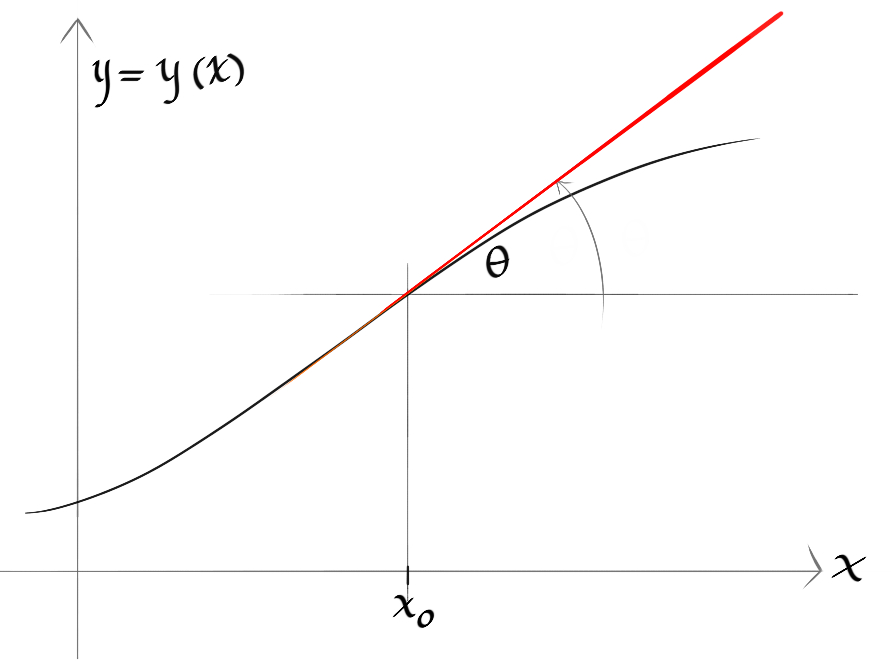
\includegraphics[width=1\textwidth]{1-significadogeom.png}
    \caption{Recta tangente en $x_0$ conocidas $\mbf{y}$ y $x_0$}\label{img:1-siggeom}
\end{subfigure}
\begin{subfigure}{.5\textwidth}
    \centering
    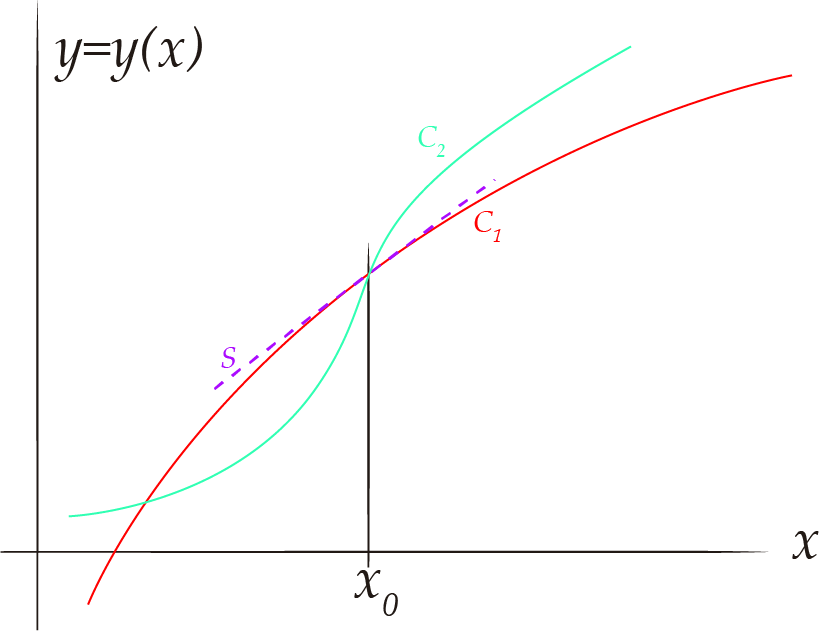
\includegraphics[width=1\textwidth]{1-significadogeom2.png}
    \caption{Curvas dadas el segmento $\mathcal{S}$.}\label{img:1-siggeom2}
\end{subfigure}
\end{figure}
Entonces, $\mbf{y'}(x_0) = \tan{\theta}$, que es la pendiente de la recta tangente a la gráfica de $\mbf{y}$ en $x_0$. Esto es cálculo elemental, lo que nos interesa es saber algo de la función $\mbf{y}$ cuando sabemos algo de $\mbf{y'}$.\\

Ilustramos en la figura \ref{img:1-siggeom2} entonces la casuística de conocer $\P \equiv \mbf{y'} = f(x,\mbf{y})$. En este caso, nos preguntamos que aspecto podría tener $\mbf{y}$ para que fuera solución de $\P$. Como conocemos $y'(x_0)$, podemos considerar que $\mathcal{S}$ es un semento paralelo a la recta tangente de la gráfica en $x_0$. Es fácil ver que $\mathcal{C}_1$ no puede ser solución de $\P$ pues $\mathcal{C}'_1(x_0) \neq y'(x_0)$. Sin embargo, es evidente que $\mathcal{C}_2$ sí resuelve $\P$.\\\\
Si repetimos el procedimiento de determinar como son las pendientes (como acabamos de hacer para $x_0$) para todos los puntos, hallamos el \textit{campo de pendientes}.

\begin{eg}[Hallar un campo de pendientes]\label{eg:campo-pendientes}
    Sea $\P \equiv \mbf{x'} = t^2 + \mbf{x}^2$, es decir, $f(t, \mbf{x}) = t^2 + \mbf{x}^2$. Si queremos hallar qué pendiente se le asigna al punto $p = (\sfrac{1}{\sqrt{2}},\sfrac{1}{\sqrt{2}})$ evaluamos la función $f$, $f(p) = 1$. Por tanto, la función $\mbf{x}$ que soluciona $\P$ tiene tangente con pendiente $1$ en $t = \sfrac{1}{\sqrt{2}}$.\\\\
    De hecho, es lógico pensar que a cualquier punto que cumpla $t^2 + \mbf{x}^2 = 1$ se le asignará una pendiente de $1$ a su recta tangente. Este conjunto de puntos conforman la \textbf{isoclina} de pendiente 1.\\\\
    De forma general, para una constante $c$ dada (en este ejemplo necesariamente no negativa pues $f(t, \mbf{x})$ es suma de cuadrados), podemos definir la isoclina de pendiente c:
    $$
    ISO_c = \left\{(t, \mbf{x}) \mid f(t, \mbf{x}) = c\right\}
    $$
    Volviendo a nuestro ejemplo, las isoclinas van a ser curvas que cumplan $t^2 + \mbf{x}^2 = c$ para un $c$ dado.\\
    \begin{minipage}[c]{0.3\linewidth}
      \begin{center}
          \raisebox{\dimexpr \topskip-\height}{
        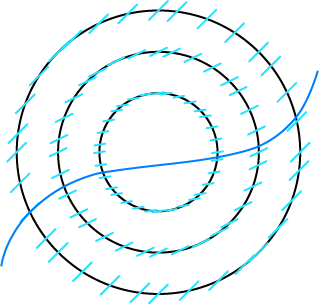
\includegraphics[width=\textwidth]{1-isoclinas.png}}
      \end{center}
    \end{minipage}\hfill
    \begin{minipage}[c]{0.65\textwidth}
        Hemos representado las isoclinas junto con un pequeño segmento de pendiente $c$ para disintos valores de $c$. Como las isoclinas cumplen que $t^2 + \mbf{x}^2 = c$, estas son las circumferencias de radio $\sqrt{c}$ con $c > 0$.\\
        Podemos observar tambien que $ISO_0 = \{(0,0)\}$ e $ISO_{c < 0} = \varnothing$.\\\\ Llamamos a la gráfica con pequeños segmentos \textit{campo de pendientes} y por tanto, una función que resuelva $\P$ tiene que ser tangente al segmento del punto por el que pase.
    \end{minipage}
    Sin embargo, los campos de pendientes permiten ver cómo es la función a grandes rasgos. En nuestro ejemplo parece indicar que $x(t) \uparrow \infty$, pero no sabemos si lo hace de forma asintótica ($x(t) \uparrow \infty$ en t finito), o x(t) crece a infinito cuando $t \rightarrow \infty$.\\
    Esto no puede resolverse gráficamente y veremos como resolverlo de forma analítica más adelante.
\end{eg}

\section{Ecuaciones diferenciales y problemas geométricos}
Gracias a la relación de la derivada con la tangencia de funciones, podemos plantear problemas geométricos en forma de ecuación diferencial.
\subsection{Trayectorias ortogonales}
De la recta tagente a un punto surge el concepto de recta normal a ese punto, que no es más que la recta perpendicular a la tangente y que pasa por dicho punto. Para ver como se relacionan estas dos rectas vamos a hacer un análisis simple. Diremos que dos curvas son ortogonales si en el punto de cruce las rectas tangentes a cada curva son perpendiculares entre sí.
\begin{wrapfigure}[20]{l}{0.5\textwidth}
  \begin{center}
    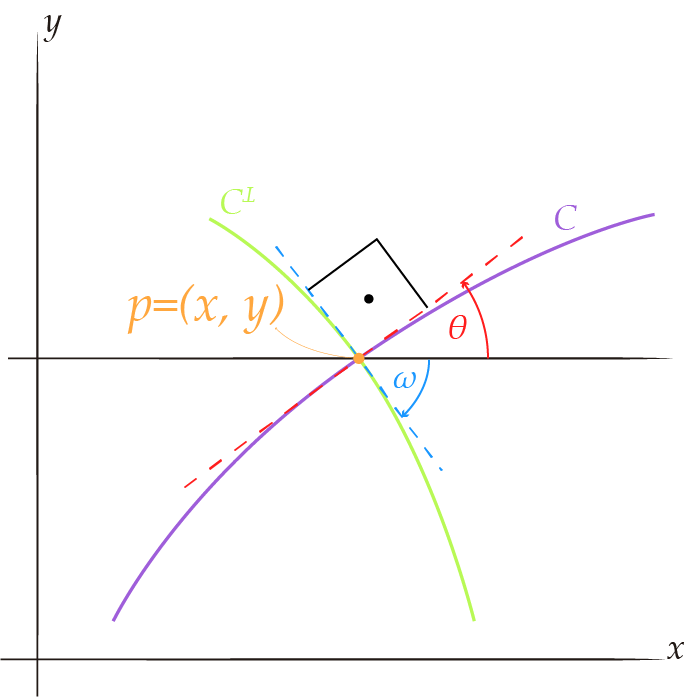
\includegraphics[width=0.48\textwidth]{1-trayectoriasortogonales.png}
  \end{center}
  \caption{Relaciones entre curvas ortogonales}\label{img:1-trayort}
\end{wrapfigure}
De la figura \ref{img:1-trayort} vemos que la pendiente de $C$ es $pend_C = \tan(\theta)$. Asimismo, $pend_{C^{\perp}} = \tan(\omega)$ y $\omega = \theta - \sfrac{\pi}{2}$. A partir de aquí desarrollamos:
$$
    \tan(\omega)=\frac{\sin(\theta-\sfrac{\pi}{2})}{\cos(\theta-\sfrac{\pi}{2})} = \frac{-\cos(\theta)}{\sin(\theta)} = -\frac{1}{\tan(\theta)}
$$
y por tanto,
\begin{equation} \label{eq:pendientes}
    pend_C \cdot pend_{C^{\perp}} = -1
\end{equation}

Nuestro objetivo es que dada una familia de curvas $fam_{C}$, podamos encontrar una (\textit{familia de}) curva que sea ortogonal a todas las de la familia en los puntos de cruce.\\\\
Supongamos que la familia original satisface una ecuación diferencial ordinaria $\mbf{y_1'} = f(x, \mbf{y_1})$. Queremos encontrar otra ecuación que defina a la ortogonal.\\\\
Como $fam_{C}$ sigue una EDO (\textit{ecuación diferencial ordinaria}), podemos afirmar que $pend_{C} = \mbf{y_1'} = f(x, \mbf{y_1})$. Usando \ref{eq:pendientes}, $pend_{C^\perp} = \frac{-1}{f(x, \mbf{y_1})}$. Pero además, si $C^\perp$ sigue una EDO, está dada por una función $\mbf{y_2} = y_2(x)$ y entonces $\mbf{y_2'} = \frac{-1}{f(x, \mbf{y_1})}$.\\
Concluimos con que dada $fam_C$ descrita por $\mbf{y'}=f(x,\mbf{y})$, podemos encontrar $fam_{C^\perp}$ que satisface:
$$
    \mbf{y'} = -\frac{1}{f(x, \mbf{y})}
$$
\begin{eg}[Familia ortogonal a otra dada]
    Consideramos la familia: $x^2-\mbf{y}^2 = c \mid c \neq 0$\\
    Para cada $c$, eso define $\mbf{y}$ implícitamente en función de $x$.
    \begin{center}
        \vspace{1mm}
        \hfill
        \begin{tikzpicture}
            \begin{axis}[domain=-5:5,samples=150,
            restrict y to domain=-5:5,
            xtick=\empty,ytick=\empty,
            %extra x ticks={0.8,1.4}, linea vertical
            %extra y ticks=3.333333,extra y tick labels={$\frac{10}{3}$}, linea horizontal
            grid=both,axis lines=middle, axis equal
            ]
                \addplot+[no marks, thick, red, solid] ({x},{x}) node[pos=0.1, below, sloped] {$c=0$};
                \addplot+[no marks, thick, red, solid] ({x},{-x});
                %%%%%%%%%%%%%%%%%%%%%%%%%%%%%%%%%%%%%%%%%%%%%%%%%%%%%%%%%%%%%%%%%%%
                \addplot+[no marks, thick, coolblack, solid] ({(x^2+1)^(1/2)},{x}) node[pos=0.5, right] {$c > 0$};
                \addplot+[no marks, thick, coolblack, solid] ({-(x^2+1)^(1/2)},{x});
                \addplot+[no marks, thick, coolblack, densely dashed] ({(x^2+4)^(1/2)},{x});
                \addplot+[no marks, thick, coolblack, densely dashed] ({-(x^2+4)^(1/2)},{x});
                \addplot+[no marks, thick, coolblack, densely dotted] ({(x^2+9)^(1/2)},{x});
                \addplot+[no marks, thick, coolblack, densely dotted] ({-(x^2+9)^(1/2)},{x});
                %%%%%%%%%%%%%%%%%%%%%%%%%%%%%%%%%%%%%%%%%%%%%%%%%%%%%%%%%%%%%%%%%%%
                \addplot+[no marks, thick, black, solid] {(x^2+1)^(1/2)} node[pos=0.5, above, sloped] {$c < 0$};
                \addplot+[no marks, thick, black, solid] {-(x^2+1)^(1/2)};
                \addplot+[no marks, thick, black, densely dashed] {(x^2+4)^(1/2)};
                \addplot+[no marks, thick, black, densely dashed] {-(x^2+4)^(1/2)};
                \addplot+[no marks, thick, black, densely dotted] {(x^2+9)^(1/2)};
                \addplot+[no marks, thick, black, densely dotted] {-(x^2+9)^(1/2)};
            \end{axis}
        \end{tikzpicture}\hfill \break
        \vspace{1pt}
        $x^2-y^2=c$ para distintos valores de $c$.\\
        (También puede verse como las curvas de nivel del paraboloide hiperbólico)
    \end{center}
    \vspace{5pt}
    Para hallar la familia de curvas ortogonales vamos a seguir una serie de pasos:
    \begin{enumerate}
        \item \texttt{Encontrar una EDO que cumplan esas curvas.}\\
            $$
                x^2-\mbf{y}^2 = c \rightarrow \Dd{x} (x^2-y^2=c) \rightarrow 2x - 2\mbf{y}\mbf{y'} = 0 \implies \mbf{y'} = \frac{x}{\mbf{y}} = f(x,\mbf{y})
            $$
        \item \texttt{Encontrar la EDO para trayectorias ortogonales.}\\
            $$
                \mbf{y'} = -\frac{1}{f(x, \mbf{y})} = -\frac{\mbf{y}}{x}
            $$
        \item \texttt{Resolver la ecuación anterior}\\
            $$
                \dd{y}{x} = -\frac{\mbf{y}}{x} \implies -\frac{\d y}{\mbf{y}} = \frac{\d x}{x} \implies \log|y| = \log|x| + \mathcal{C}
            $$
            es decir,
            $$
                |\mbf{y}| = \frac{e^\mathcal{C}}{|x|} \implies |x\mbf{y}| = e^\mathcal{C} \implies x\mbf{y} = k : k = e^\mathcal{C} \lor k = e^{-\mathcal{C}} \implies \mbf{y} = \frac{k}{x}
            $$
    \end{enumerate}
    Con la solución general podemos representar parte de la familia:
    \begin{center}
        \vspace{1mm}
        \hfill
        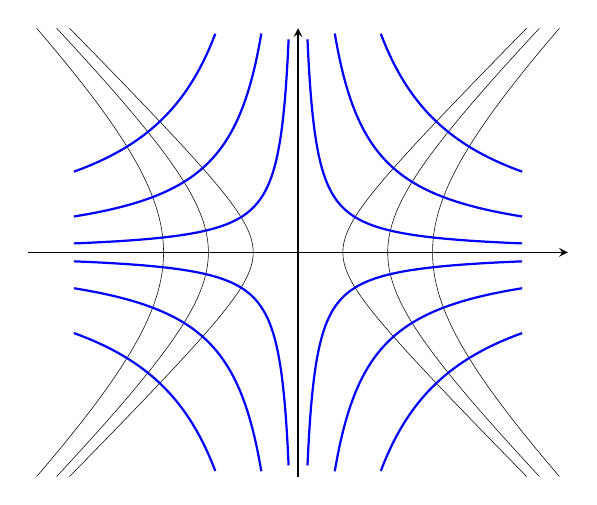
\begin{tikzpicture}
            \begin{axis}[domain=-5:5,samples=150,
            restrict y to domain=-5:5,
            xtick=\empty,ytick=\empty,
            %extra x ticks={0.8,1.4}, linea vertical
            %extra y ticks=3.333333,extra y tick labels={$\frac{10}{3}$}, linea horizontal
            grid=both,axis lines=middle, axis equal
            ]
                \addplot+[no marks, very thin, black, solid] ({(x^2+1)^(1/2)},{x});
                \addplot+[no marks, very thin, black, solid] ({-(x^2+1)^(1/2)},{x});
                \addplot+[no marks, very thin, black, solid] ({(x^2+4)^(1/2)},{x});
                \addplot+[no marks, very thin, black, solid] ({-(x^2+4)^(1/2)},{x});
                \addplot+[no marks, very thin, black, solid] ({(x^2+9)^(1/2)},{x});
                \addplot+[no marks, very thin, black, solid] ({-(x^2+9)^(1/2)},{x});
                %%%%%%%%%%%%%%%%%%%%%%%%%%%%%%%%%%%%%%%%%%%%%%%%%%%%%%%%%%%%%%%%%%%
                \addplot+[no marks, thick, blue, solid, samples=500] {1/x};
                \addplot+[no marks, thick, blue, solid, samples=500] {-1/x};
                \addplot+[no marks, thick, blue, solid, samples=300] {4/x};
                \addplot+[no marks, thick, blue, solid, samples=300] {-4/x};
                \addplot+[no marks, thick, blue, solid] {9/x};
                \addplot+[no marks, thick, blue, solid] {-9/x};
            \end{axis}
        \end{tikzpicture}\hfill \break
        \vspace{1pt}
        En azul posibles soluciones para disintos valores de $k$, en negro la familia original\\
        Se observa que son curvas ortogonales a la familia original.
    \end{center}
\end{eg}

\subsection{Trayectorias ortogonales en coordenadas polares}
Veamos que al igual que encontramos una expresión para la trayectorias ortogonales en coordenadas rectangulares, también lo podemos hacer en coordenadas polares. En este caso partimos de una familia de curvas $fam_C$ descrita por la solución de una EDO $\mbf{r'} = h(\mbf{r}, \theta)$. ¿Cuál es la familia ortogonal $fam_{C^\perp}$?.\\\\
Para ello tenemos que empezar analizando la expresión de la tangente como ecuación.

\begin{wrapfigure}{l}{.6\textwidth}
  \begin{center}
    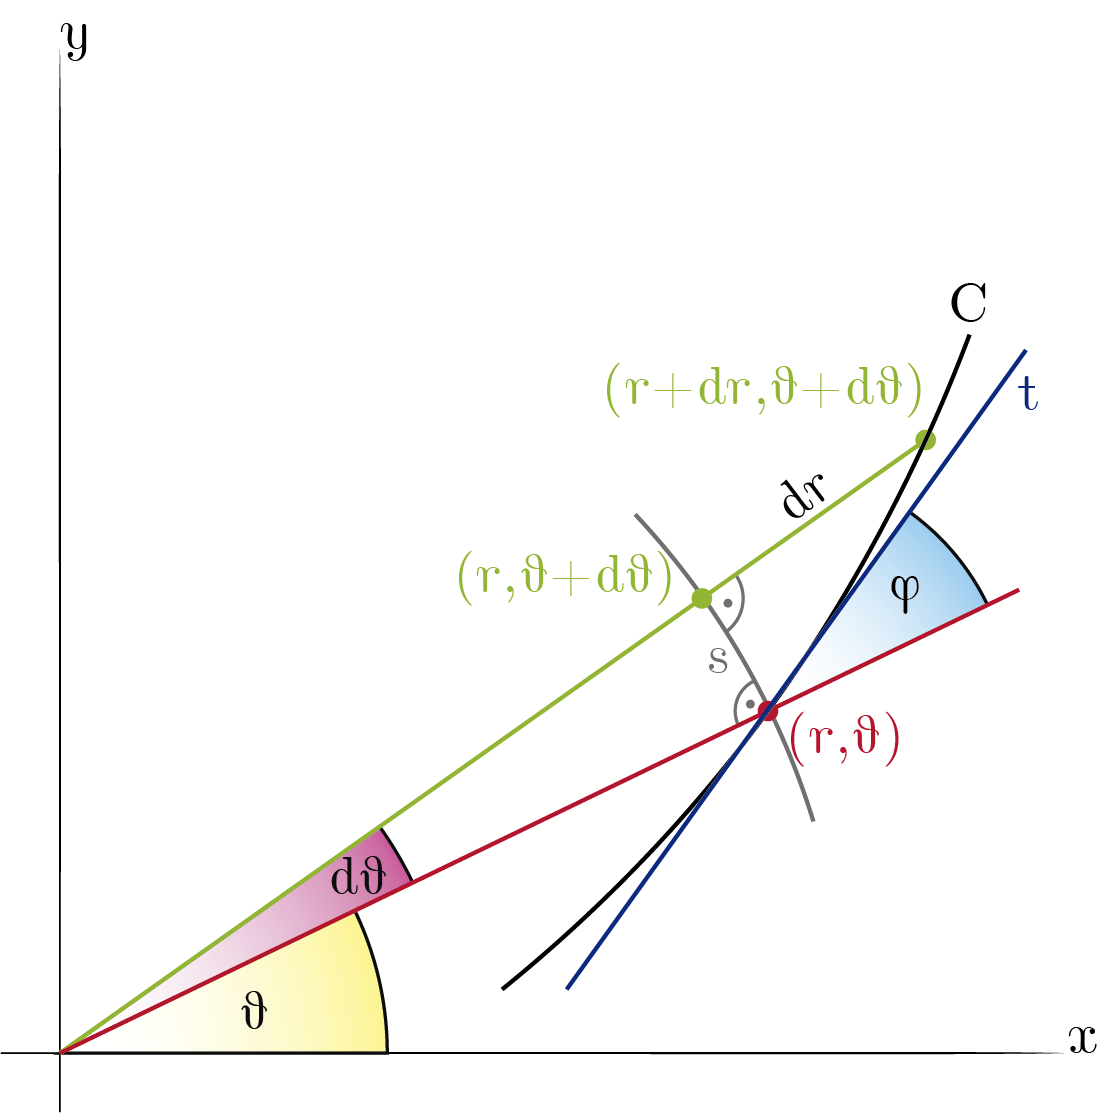
\includegraphics{1-ortogonalpolares.png}
  \end{center}
  \caption{Analisis de $\d r$ y $\d \theta$}\label{img:1-polort}
\end{wrapfigure}
En la figura \ref{img:1-polort} hemos trazado una curva arbitraria $C$. Queremos hallar una ecuación diferencial que describa a la tangente en cierto punto $p = (r,\theta)$. Para ello, hallamos un nuevo punto $q = (r + \d r, \theta +\d \theta) \in C$. Se indica además la cirfumferencia $s$ de radio $r$ con centro en $0$, y la recta tangente $t$ al punto original $p$.\\\\
Observamos que $s$ es perpendicular a las rectas que unen el origen con $p$ y $q$ ($\vec{0p}$ y $\vec{0q}$ respectivamente), ya que son trazadas desde el radio de la misma. Además, la intersección de $\vec{0q}$ con $s$ nos marca el punto $q' = (r, \theta +\d \theta)$. Finalmente, denominamos $\phi$ al ángulo del que queremos hallar la tangente.

El gráfico de la figura \ref{img:1-polort} está distorsionado. Tanto $\d r$ como $\d \theta$ son infinitesimales, es decir, extremadamente pequeños. Debido a ello podemos hacer distintas asunciones.\\\\
Para comenzar, el arco de circumferencia que une $p$ y $q'$ tiene longitud $r\d \theta$ y podemos aproximarlo con un segmento que va a ser perpendicular a las rectas $\vec{0p}$ y $\vec{0q}$. Esto hará que $\vec{0p}$ y $\vec{0q}$ sean aproximadamente paralelas, pues comparten un mismo segmento perpendicular a ellas.\\ Además, podemos aproximar el arco de $C$ que une $p$ y $q$ con un segmento de $t$. Esto se ilustra en la figura \ref{img:1-polort2}.

\begin{wrapfigure}{r}{.5\textwidth}
  \begin{center}
    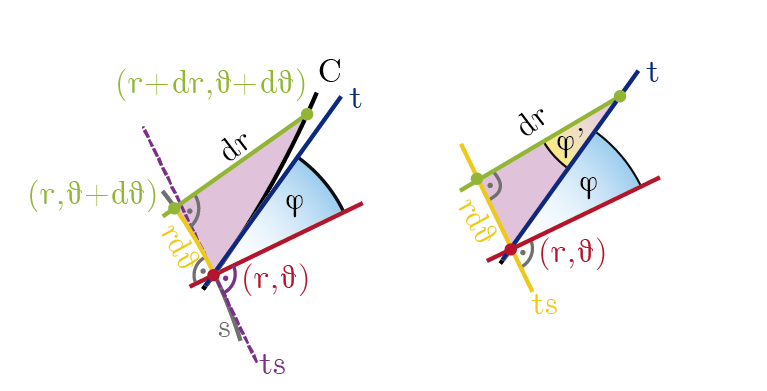
\includegraphics[scale=1.2]{1-ortogonalpolares2.png}
  \end{center}
  \caption{Aproximación por infinitesimales}\label{img:1-polort2}
\end{wrapfigure}

Como puede apreciarse en \ref{img:1-polort2}, el área sombreada se corresponde con un triangulo rectángulo en la aproximación, y de hecho tenemos descritos los catetos, lo que nos permite hallar $\tan\phi'$. Sin embargo, como hemos visto en la aproximación, ambas rectas perpendiculares a $ts$ son paralelas entre sí. Es fácil ver entonces que $\phi = \phi'$ y al describir $\tan\phi'$ hemos descrito $\tan\phi$.\\\\
Por tanto, podemos concluir que:
$$
\tan\phi = \frac{r\d \theta}{\d r} = r \frac{1}{\dd{r}{\theta}} = \frac{r}{r'}
$$
Una vez hemos descrito la forma que tiene la tangente a una curva $C$ arbitaria en forma de ecuación diferencial $r' = h(r,\theta)$, podemos hallar $fam_{C^\perp}$ que buscábamos al comienzo de la sección. Para ello, vamos a considerar de nuevo una curva arbitraria $C$ y su perpendicular $C^\perp$. Nos interesa especialmente la relación que existe entre los ángulos de las rectas tangentes de cada curva.\\\\
\begin{wrapfigure}{r}{.5\textwidth}
  \begin{center}
    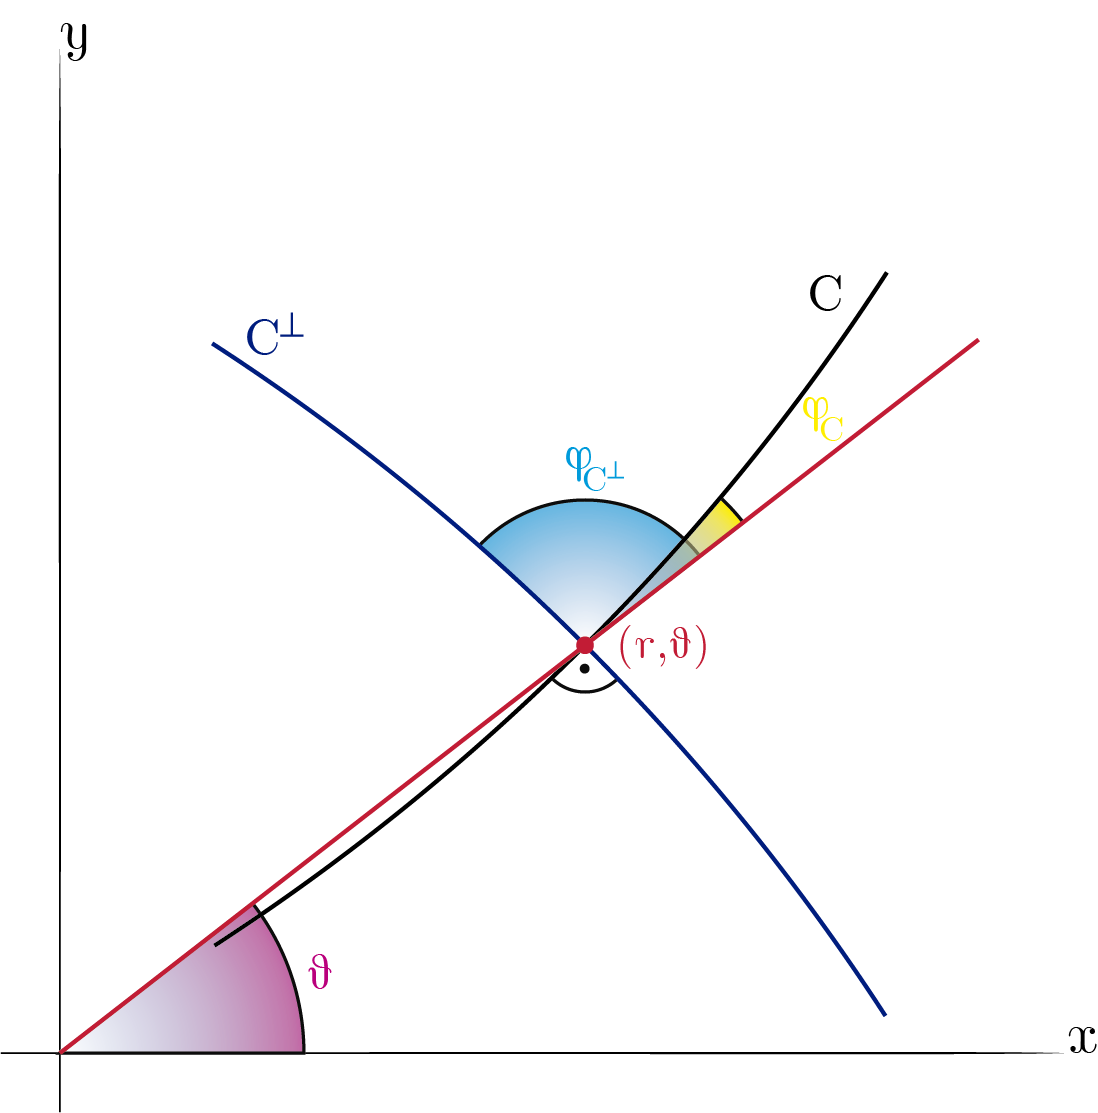
\includegraphics[scale=1]{1-ortogonalpolares3.png}
  \end{center}
  \caption{Angulos entre curvas ortogonales}\label{img:1-polort3}
\end{wrapfigure}

En la figura \ref{img:1-polort3} se ilustra la relación que buscamos. Supongamos que las dos curvas se cortan en un punto $p = (r, \theta)$ y consideramos la recta $\vec{0p}$. Al igual que en la figura \ref{img:1-polort}, definimos $\phi_C$ como el ángulo existente entre $\vec{0p}$ y la curva $C$. Siguiendo el mismo procidimiento podemos definir $\phi_{C^\perp}$.\\
Como por definición $C \perp C^{\perp}$, entonces el ángulo existente entre ellas es $\sfrac{\pi}{2}$, por tanto: $\phi_{C^\perp} = \sfrac{\pi}{2} + \phi_C$.\\\\
Del caso en coordenadas rectangulares recordamos la ecuación:
$$
\tan(\phi_{C^\perp}) = -\frac{1}{ \tan(\phi_C)}
$$
donde a la derecha de la ecuación figura todo lo relacionado con la curva original y a la izquierda lo relacionado con la curva tangente. Como hallamos antes que $\tan\alpha = \sfrac{r}{r'}$ para un ángulo $\alpha$ que describa a la recta tangente, de la misma forma $\tan(\phi_{C^\perp}) = \sfrac{r}{r'}$ describe a su recta tangente, que es ortogonal a la curva $C$ original.\\ Usando esto, la definición $r' = h(r, \theta)$ del comienzo de la sección y la ecuacion anterior obtenemos:
$$
\frac{r}{r'} = -\frac{1}{\sfrac{r}{r'}} = -\frac{1}{\sfrac{r}{h(r,\theta)}} \implies \frac{r}{r'} = -\frac{h(r,\theta)}{r}
$$
Finalmente, de la expreisón anterior hallamos la ecuación diferencial general para describir a $fam_{C^\perp}$ a partir de la función $h(r, \theta)$ que describe a $fam_C$:
$$
    r' = -\frac{r^2}{h(r, \theta)}
$$
\section{Ecuaciones homogéneas de grado 0}
En esta sección daremos un breve método para resolver ecuaciones homogéneas de grado $0$.
\begin{dfn}[Ecuación homogénea de grado k]
    Sea $f: \matbb{K} x \matbb{K} \longrightarrow \matbb{K}$, decimos que es \textbf{homogénea de grado k} $\iff f(\lambda x_1, \lambda x_2) = \lambda^k \cdot f(x_1, x_2)$
\end{dfn}
Nos interesarán especialmente las de grado $k=0$, es decir, aquellas en que $f(\lambda x_1, \lambda x_2) = f(x_1, x_2)$.\\\\
Supongamos que tenemos la EDO $\mbf{y'} = f(x, \mbf{y})$, tenemos que $f(x, \mbf{y}) = f(x, \mbf{y} \cdot \sfrac{x}{x})$. Si $f$ es homogénea de grado 0, y tomamos $\lambda = x$ entonces, $f(x, \mbf{y} \cdot \sfrac{x}{x}) = f(\lambda, y \cdot \sfrac{\lambda}{x}) = \lambda^0 f(1, \sfrac{\mbf{y}}{x})$, es decir:
$$
    \mbf{y}' = f(x,\mbf{y}) = f\left(1, \frac{\mbf{y}}{x}\right)
$$
Haciendo el cambio $\mbf{z} = \sfrac{\mbf{y}}{x}$ y desarrollando $\mbf{z'}$ tenemos:
$$
    \mbf{z'} = \frac{\mbf{y'}}{x} - \frac{\mbf{y}}{x} = \frac{f\left(1,\frac{\mbf{y}}{x}\right)}{x} - \frac{1}{x} \frac{\mbf{y}}{x} = \frac{f(1,\mbf{z}) - \mbf{z}}{x}
$$
que es una EDO de variables separables.\\Veamos un ejemplo con resolución por este método:
\begin{eg}[Espejo parabólico]
    Queremos construir un espejo para los faros de un automóvil. Buscamos que si la luz proviene del origen (la bombilla), ésta salga reflejada paralela al suelo. Vamos a hallar qué forma tiene que tener una sección del espejo (que tiene simetría radial) que cumple nuestro objetivo. Vamos a ejemplificar con la ayuda del diagrama siguiente.\\
    \begin{minipage}[c]{0.5\linewidth}
      \begin{center}
          \raisebox{\dimexpr \topskip-\height}{
        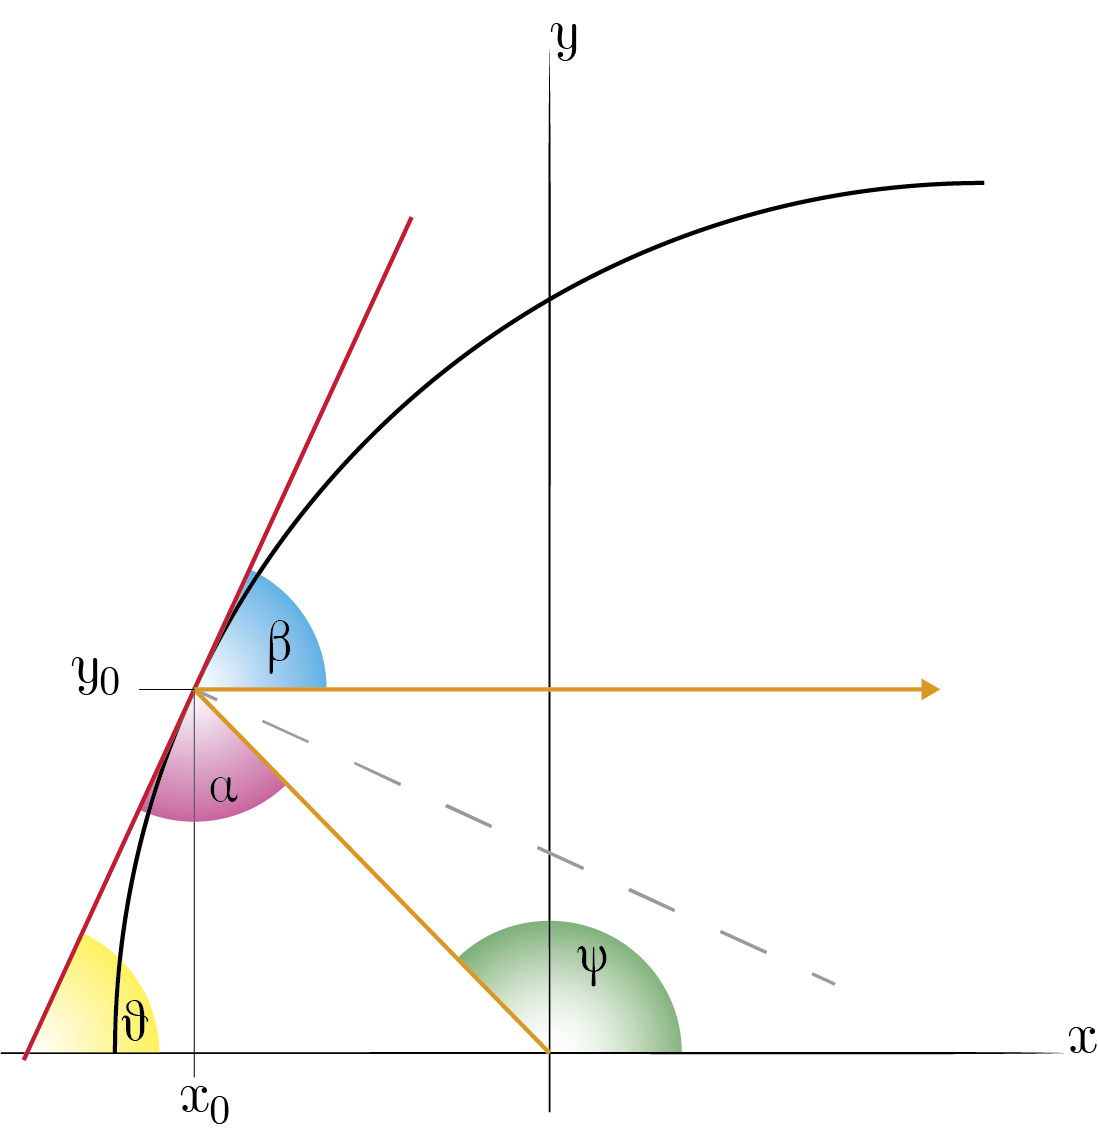
\includegraphics[width=\textwidth]{1-espejo.png}}
      \end{center}
    \end{minipage}\hfill
    \begin{minipage}[c]{0.45\textwidth}
        En la figura hemos marcado 4 ángulos: $\alpha$, $\beta$, $\theta$ y $\psi$.\\ Si nos fijamos con más detenimiento, como la trayectoria del rayo es paralela al eje $X$ los ángulos que forman ambas con la recta tangente en un punto arbitrario del espejo son idénticos, por lo que $\beta = \theta$.\\ Además, debido a que en la reflexión de un haz de luz el ángulo de reflexión coincide con el de incidencia tenemos que $\alpha = \beta$.\\ Es fácil ver que el ángulo suplementario a $\psi$ ($\pi - \psi\ rad$) forma parte de los ángulos internos de un triángulo, junto con $\alpha$ y $\theta$. Por ello, podemos expresar la igualdad $\alpha + \theta + (\pi - \psi) = \pi\ rad \implies \psi = \alpha + \theta = 2\theta$.
    \end{minipage}
    Como ya viene siendo conocido, $\tan(\theta) = \mbf{y}'$. Y si nos fijamos en la figura, para cualquier punto $(x,\mbf{y})$ del espejo $\tan(\psi) = \sfrac{\mbf{y}}{x}$. Por tanto:
    $$
        \frac{\mbf{y}}{x} = \tan(\psi) = \tan(2\theta) = \frac{\sin(2\theta)}{\cos(2\theta)} = \frac{2\sin(\theta)\cos(\theta)}{\cos^2(\theta)-\sin^2(\theta)} = \frac{2\tan(\theta)}{1-\tan^2(\theta)} = \frac{2\mbf{y'}}{1-\mbf{y'}^2}
    $$
    es decir,
    $$
        (1-\mbf{y'}^2)\cdot \mbf{y} = 2\mbf{y'}\cdot x \implies \mbf{y'} = \frac{-x \pm (x^2+\mbf{y}^2)^{\sfrac{1}{2}}}{\mbf{y}}
    $$
    de las dos opciones que tenemos, tenemos que ver cuál es válida. Como la pendiente de la recta tangente es positiva, nuestra ecuación diferencial sólo puede ser:
    $$
        \mbf{y'} = \frac{-x + \sqrt{(x^2+\mbf{y}^2)}}{\mbf{y}}
    $$
    Salta a la vista que no podemos resolverla por el método de separación de variables. Por ello, vamos a considerar un cambio de variables para convertirla en una ecuación de variables separables.\\\\
    Sea $z(x) = \sfrac{y(x)}{x}$, hallamos la expresión de $\mbf{z'}$:
    $$
        \mbf{z'} = \frac{\mbf{y'}}{x} - \frac{\mbf{y}}{x^2} = \frac{1}{x} \cdot (\mbf{y'} - \mbf{z}) = \frac{1}{x} \cdot \left(\frac{-x + \sqrt{(x^2+\mbf{y}^2)}}{\mbf{y}} - \mbf{z}\right) = \frac{1}{x} \cdot \left(-\frac{x}{\mbf{y}} +\sqrt{\left(\frac{x}{\mbf{y}}\right)^2+1} -\mbf{z}\right)
    $$
    y si del último paso hacemos el cambio $\sfrac{1}{\mbf{z}} = \sfrac{x}{\mbf{y}}$ obtenemos:
    $$
        \mbf{z'} = \frac{1}{x} \cdot \left(-\frac{1}{\mbf{z}} + \sqrt{\frac{1}{\mbf{z}^2}+1} - \mbf{z} \right)
    $$
    que es de variables separables.\\\\
    La solución a esta EDO es: $1 - \sqrt{1+\mbf{z}^2} = \frac{c}{x}$ y como $\mbf{z} = \sfrac{\mbf{y}}{x}$ obtenemos la ecuación que describe la altura de nuestro espejo en función de $x$ y una constante $c$, a falta de algún dato extra para resolver un PVI.
    $$
        y(x) = \sqrt{c^2 + 2cx}
    $$
\end{eg}

\section{Ecuaciones lineales de orden I}
Vamos a ver un nuevo tipo de ecuaciones que no se pueden resolver por los métodos anteriormente descritos, sin embargo, vamos a comenzar ejemplificando el tipo de ecuación para enunciar una proposición más adelante.

\begin{eg}[Ecuaciones lineales de orden I - Intuición]\label{eg:lineal-order}
    Sea $\mathcal{(EC)} \equiv \mbf{x'} = \mbf{x} + t$, vamos a intentar resolverla, es decir, queremos encontrar una expresión para x(t).\\
    \begin{enumerate}
        \item Vamos a considerar primero la ecuación sin el término que únicamente depende de $t$ : $\mbf{x}' = \mbf{x}$. En este caso es sencillo ver que $e^t$ es solución.

        \item Consideramos ahora $y(t) = e^{-t}x(t)$, donde $x(t)$ es solución de $\mathcal{(EC)}$ (como observación, $e^-t$ es la inversa de la solución encontrada en (1)). Derivando se obtiene que:
        $$
            y'(t) = -e^{-t}\cdot \mbf{x} + e^{-t} \cdot \mbf{x'} = e^{-t} \cdot (\mbf{x'}  - \mbf{x}) = t \cdot e^{-t}
        $$
        Solo queda integrar y despejar $x(t)$ de $y(t) = \int y'(t)$:
        $$
            y(t) = \int y'(t) \d t = \int t \cdot e^{-t} \d t = -te^{-t} - e^{-t} + C,\ C\ constante
        $$
        es decir,
        $$
            e^{-t} \cdot x(t) = -te^{-t} - e^{-t} + C \implies x(t) = Ce^t - 1 - t
        $$
    \end{enumerate}
    Con lo que hemos hallado la solución general a nuestra ecuación.
\end{eg}
\begin{obs}
    Veamos ciertos aspectos de lo que hemos hallado.\\
    \begin{enumerate}
        \item $(-1-t)$ es una solución particular de $\mathcal{(EC)}$ (cuando $C=0$).
        \item $e^t$ es solución de la \textit{ecuación homogénea} $\mbf{x'} = \mbf{x}$.
        \item Esa ecuación homogénea es lineal, es decir, la suma de ecuaciones es solución, y por tanto la multipliación por un escalar también lo es.
        $$
        \begin{cases}
            \mbf{x'} = \mbf{x}\\ \mbf{y'} = \mbf{y}
        \end{cases}
        \implies (\mbf{x}+\mbf{y})' = \mbf{x} + \mbf{y}
        $$
        y además, si $x(t)$ es solución, $\lambda x(t)$ también lo es.
        \item Todas las solución de $\mbf{x'} = \mbf{x}$ (la homogénea) son $x(t) = Ce^t$.
        \item $x(t) = Ce^t - 1 - t$ nos dice que la solución general a $\mathcal{(EC)}$ es igual a una solución particular $(-1-t)$ más la solución de la homogénea.
    \end{enumerate}
\end{obs}
Lo que hemos hecho ha sido encontrar una solución de una ecuación del tipo $\mbf{x'} = \alpha(t)\cdot\mbf{x}+\beta(t)$ (con $\alpha(t) = 1,\ \beta(t) = t)$). Para resolver este tipo de ecuaciones enunciamos la siguiente proposición:

\begin{pro}
    Sean $\alpha,\ \beta:\ [a,b] \longrightarrow \R$ funciones continuas. Y sean:
    \begin{gather*}
        A(t) = \int_a^t \alpha(u) \d u \ \ \ \ H(t) = \int_a^t e^{-A(u)} \beta(u) \d u
    \end{gather*}
    Entonces:
    \begin{enumerate}
        \item $x(t)$ verifica $x'(t) = \alpha(t)x(t)+\beta(t)\ \forall t \in [a,b] \iff \exists c \in \R : x(t) = H(t) \cdot e^{A(t)} + c \cdot e^{A(t)}$
        \item Dados $t_0 \in (a,b)$, $x_0 \in \R$ entonces $\exists ! c : x(t) = H(t) \cdot e^{A(t)} + c \cdot e^{A(t)}$ es solución del PVI:
        $$
            \begin{cases}
                x'(t) = \alpha(t)\cdot x(t) + \beta(t)\\
                x(t_0) = x_0
            \end{cases}
        $$
    \end{enumerate}
\end{pro}
\begin{proof}
    Vamos a demostrar $1$ y $2$ por separado:
    \begin{enumerate}
        \item Tenemos $\mathcal{(EC)} \equiv x'(t) = \alpha(t)x(t) + \beta(t)$ con $\alpha, \beta$ continuas.\\
        La ecuación homogénea asociada a $\mathcal{(EC)}$ es $x'(t) = \alpha(t)x(t)$ que es lineal, es decir, la suma de soluciones es solución. Tenemos:
        $$
        \begin{cases}
            x_1'(t) = \alpha(t)x_1(t)\\
            x_2'(t) = \alpha(t)x_2(t)
        \end{cases} \implies (\mbf{x_1} + \mbf{x_2})' = \alpha(t)\cdot(\mbf{x_1} + \mbf{x_2})
        $$
        \begin{obs}
            Si sumo soluciones de $\mathcal{(EC)}$ obtengo $(\mbf{x_1} + \mbf{x_2})' = \alpha(t)\cdot(\mbf{x_1} + \mbf{x_2}) + 2\beta(t)$
        \end{obs}
        Para hallar la solución general vamos a proceder de forma parecida al ejemplo \ref{eg:lineal-order}. Sea $A(t)$ tal que $A'(t) = \alpha(t)$, entonces $x(t) = e^{A(t)}$ verifica la ecuación homogénea.\\\\
        Construimos $y(t) = e^{-A(t)}\cdot\mbf{x}$, y la igualamos con la integral de su derivada:
        $$
            (e^{-A(t)}\cdot\mbf{x})' = e^{-A}\mbf{x'} - e^{-A}\cdot \mbf{x} \cdot A' = e^{-A} \cdot (\mbf{x'} - \alpha \mbf{x}) = e^{-A} \cdot \beta
        $$
        entonces,
        $$
            y(t) = e^{-A(t)} \cdot x(t) = \int e^{-A(t)}\cdot\beta(t) \d t \implies e^{-A(t)} \cdot x(t) = H(t) + C \implies x(t) = e^{A(t)} \cdot (H(t) + C)
        $$
        \item $x_0 = x(t_0) = c\cdot e^{A(t_0)} + e^{A(t_0)} \cdot H(t) \implies \exists ! c$ pues $e^{A(t_0)} \neq 0$. Y por tanto, para el PVI:
        $$
            \begin{cases}
                x'(t) = \alpha(t)\cdot x(t) + \beta(t)\\
                x(t_0) = x_0
            \end{cases}
        $$existe solución y es única.
    \end{enumerate}
\end{proof}

\begin{eg}[Resolución ecuación lineal de orden I]
    Sea $y'(x) = x^3 - 2x\cdot y(x)$, donde $\beta(x) = x^3$ y $\alpha(x) = 2x$. Queremos hallar la expresión de todas las posibles soluciones, es decir, la solución general.\\\\
    \begin{enumerate}
        \item \texttt{Solución general de la homogénea}\\\\
        La ecuación de la homogénea es $\mbf{y}'=-2x\mbf{y}$. Es de variables separables, resolviendo obtenemos:
        $$
            y(x) = C \cdot e^{-x^2} : C \text{ es constante.}
        $$
        \item \texttt{Tomando $e^{-x^2}$ una solución de (1)}\\\\
        Volvemos a la ecuación $\mbf{y}' = x^3-2x\mbf{y}$. Por tanto, podemos reescribir $\mbf{y}' como: 2x\mbf{y} + \mbf{y}' = x^3$.\\
        A continuación, hacemos el cambio
        $$
            z(x) = e^{-(-x^2)} y(x) = e^{x^2} \mbf{y} \text{ y hallamos $z'(x)$.}
        $$
        $$
            \mbf{z}' = 2x\mbf{y}e^{x^2} + e^{x^2} = e^{x^2}\cdot (2x\mbf{y}+\mbf{y}') = e^{x^2} x^3.
        $$
        Hallamos $z(x)$ integrando $\mbf{z}'$:
        $$
            z(x) = \int x^3 e^{x^2} \d x = \frac{x^2-1}{2} \cdot e^{x^2} + C.\text{ (se resuelve por partes).}
        $$
        Igualando a nuestra $z(x) = e^{x^2} \mbf{y}$ original, despejamos $y(x)$:
        $$
            y(x) = \frac{x^2-1}{2} + C e^{-x^2}
        $$
        Donde $\frac{x^2-1}{2}$ coincide con una solución particular con $C = 0$, y $C e^{-x^2}$ es la solución general de la homogénea.
    \end{enumerate}
\end{eg}
%%Considerar si añadir la primera parte de la clase del 05/02
\section{Teoremas de existencia y unicidad}
En la sección anterior hemos enunciado una preposición que denominamos de \texit{existencia y unicidad} para ecuaciones lineales de orden I. Nos gustaría dar condiciones más genereales para saber si existen y son únicas ciertas soluciones.\\
Consideraremos el PVI general:
$$
    \begin{cases}
        \mbf{x'} = f(t, \mbf{x}) \\ x(t_0) = t_0
    \end{cases}
$$
\begin{thm}[Existencia y unicidad global]
    Sea $f: [a,b] \subset \R \longrightarrow \R$, con $f \in C^1$.\\Si $\dd{f}{x} = f_x$ es acotada,  es decir:
    $$
        \exists L \in \R : |f_x(t, \mbf{x})| \leq L\ \forall t\in[a,b],\ \forall x\in R
    $$ entonces, el PVI tiene solución y es única.
\end{thm}
La demostración la veremos más adelante cuando cosideremos el caso \texit{n-dimensional}.

\begin{obs}
    Vamos a ver ciertos aspectos de este resultado.\\
    \begin{enumerate}
        \item  Gráfica de la solución\\
        \begin{minipage}[c]{0.5\linewidth}
          \begin{center}
              \raisebox{\dimexpr \topskip-\height}{
            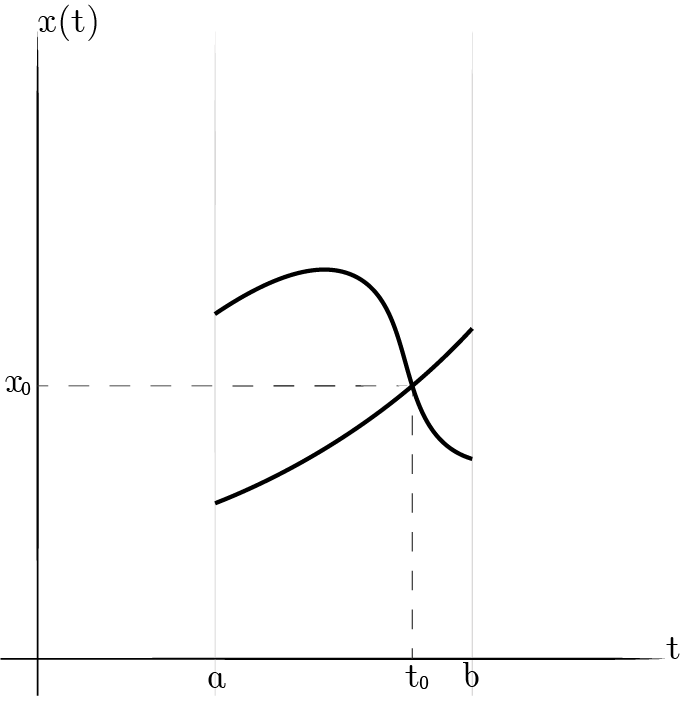
\includegraphics[width=\textwidth]{1-existencia-unicidad.png}}
          \end{center}
        \end{minipage}\hfill
        \begin{minipage}[c]{0.45\textwidth}
            A nivel visual, no puede haber dos soluciones como las de la figura. Si las hubiera, el PVI tendría dos soluciones distintas para $t_0$ y habíamos dicho que era única.\\\\
            Analíticamente podemos considerar el gráfico de $x(t)$ como un subconjunto del plano $\R^2$. Si consideramos cada solución de esta forma, digamos $S_1, S_2$, entonces:
            $$
                S_1 \cap S_2 \neq \varnothing \iff S_1 = S_2
            $$
        \end{minipage}
        \item Unicidad en la recta real\\
        \begin{minipage}[c]{0.5\linewidth}
          \begin{center}
              \raisebox{\dimexpr \topskip-\height}{
            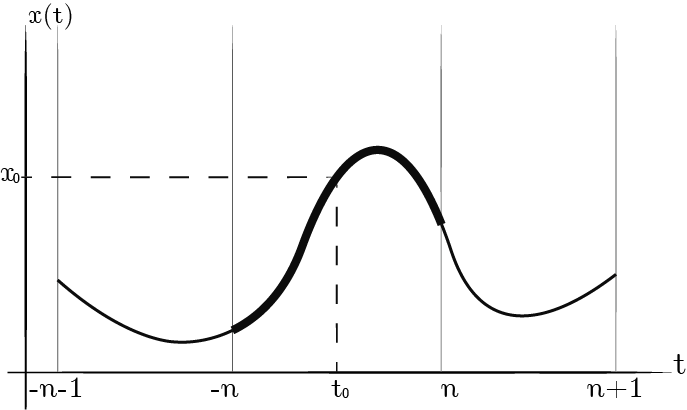
\includegraphics[width=\textwidth]{1-extension-unicidad.png}}
          \end{center}
        \end{minipage}\hfill
        \begin{minipage}[c]{0.45\textwidth}
            Sea $f: \R \times \R \longrightarrow \R$ cumple que $|f_x \leq L|$ (su derivada está acotada), entonces el PVI:
                $$
                    \begin{cases}
                        \mbf{x'} = f(t, \mbf{x})\\
                        x(t_0) = x_0
                    \end{cases}
                $$
            entonces tiene solución y es única $ \forall t \in \R$\\\\
            Si nos fijamos en la imagen de la izquierda, la idea intuitiva surge de tener una solución $x(t)$ definida sobre un intervalo $[-n, n]$. Si podemos extender $x(t)$ a $[-n-1, n+1]$, ésta tiene que coincidir en $[-n,n]$ y por unicidad, la solución es la misma. Podemos hacer esto para cualquier intervalo mayor que $[-n,n]$ y por tanto sobre la totalidad de $\R$.\\Formalemente puede intentar demostrarse por inducción sobre el tamaño del intervalo.
        \end{minipage}
        %% Mirar si introducir el ejemplo de mi página 19. Parece repetido.
    \end{enumerate}
\end{obs}
\begin{th_ex}
    Supongamos que $x(t)$ resuelve $\mbf{x'} = f(x)$ y $\lim_{t \to \infty} x(t) = a$. ¿Podemos asegurar que $f(a) = 0$?.\\ \textit{Pista:} tener en cuenta que el recíproco es cierto. Es decir, si $f(a) = 0$ entonces sabemos que hay ecauciones que se acercan a $a$ conforme avanzan.
\end{th_ex}
La versión global del teorema de existencia y unicidad no es muy útil. Veamos dos situaciones simples en las que no funciona.\\\\
Sea el PVI:
$$
    \begin{cases}
        \mbf{x'} = \mbf{x}^2\\
        x(0)=1
    \end{cases} t\in [-2,2] \text{ no tiene solución.} \label{eg:no-solution}
$$
Si intentamos resolverlo:
\begin{gather*}
    \dd{x}{t} = \mbf{x}^2 \implies \int \frac{\d x}{\mbf{x}^2} = \int \d t \implies -\frac{1}{\mbf{x}} = t + C\\
    x(0) = 1 \implies C = -1 \implies x(t) = \frac{1}{1-t}
\end{gather*}
que no es solución en $[-2,2]$ pues no está definida para $t=1$.\\\\

\begin{wrapfigure}[12]{r}{0.6\textwidth}
  \begin{center}
    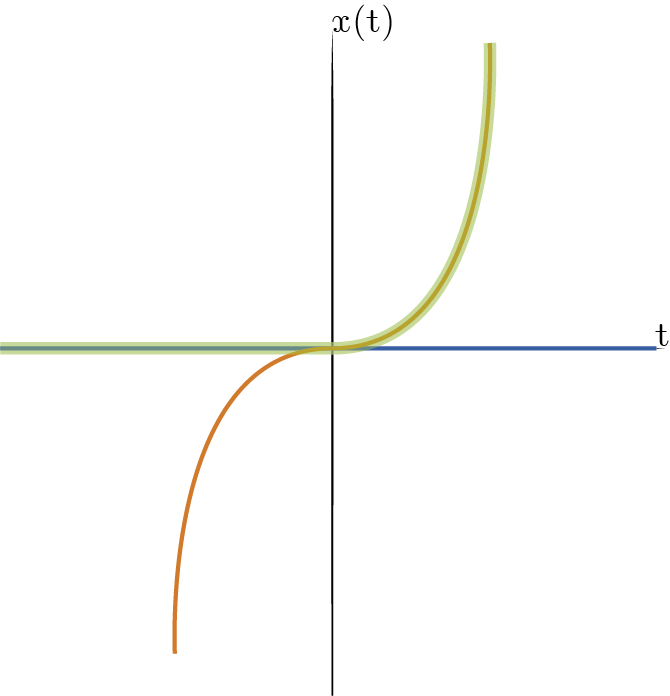
\includegraphics[width=0.4\textwidth]{1-no-unicidad.png}
  \end{center}
  \caption{Solución no única}\label{img:1-no-unicidad}
\end{wrapfigure}
Consideremos ahora el PVI:
$$
    \begin{cases}
        \mbf{x'} = \mbf{x}^{\sfrac{2}{3}}\\
        x(0)=0
    \end{cases}
$$
es facil ver que tanto $x_1(t) = 0$ como $x_2(t)=(\frac{t}{3})^3$ resuelven el PVI. De hecho, si combino trozos de la función puedo hallar más. En la figura se representan ambas soluciones y se resalta una posible combinación.\\\\

\begin{thm}[Existencia y unicidad local]
    Sean $[a,b] \times [c,d] = A \subset \R \times \R$, una función $f: A \longrightarrow \R$ con $f \in C^1$ y $t_0\in(a,b)$, $x_0\in(c,d)$. Entonces:\\
    \begin{itemize}
        \item Existencia:\\
            $
                \exists \delta > 0 \text{ y } x:(t_0 - \delta, t_0 + \delta) \longrightarrow \R, \mbf{x}\in C^1
            $ tal que $\mbf{x}$ es solución del PVI:
            $$
                \begin{cases}
                    \mbf{x'} = f(t, \mbf{x})\\
                    x(t_0) = x_0
                \end{cases}
                \text{con } \delta < \min(t_0 - a, b - t_0)
            $$
        \item Unicidad:\\
        Si $x_1(t)$, $x_2(t)$ son $C^1$ en un intervalo $(t_0-\varepsilon, t_0+\varepsilon)$ y satisfacen:\\
        $$
            \begin{cases}
                \mbf{x_i'} = f(t, \mbf{x_i}),\ |t-t_0| < \varepsilon\\
                x_i(t_0) = x_0
            \end{cases}
            \text{con } \varepsilon < \min(t_0 - a, b - t_0)
        $$ entonces $x_1(t) = x_2(t)\ \forall t : |t-t_0| < \varepsilon$.
    \end{itemize}
\end{thm}
De nuevo, se deja la demostración para cuando enunciemos el caso \textit{n-dimensional}.
\begin{obs}
    Al igual que en el caso global, vamos a estudiar una serie de implicaciones de este resultado.\\
    \begin{enumerate}
        \item Unicidad local.\\
        Podemos expresar la solución analíticamente como:\\\\
        Sean $x_1(t),\ x_2(t)$ soluciones a un PVI. Si $x_1(t_0) = x_2(t_0)$, entonces $ \exists \varepsilon>0: x_1(t) = x_2(t),\ \forall t : |t-t_0| < \varepsilon$
        \item Prolongación de la solución.\\
        \begin{center}
            \raisebox{\dimexpr \topskip-\height}{
          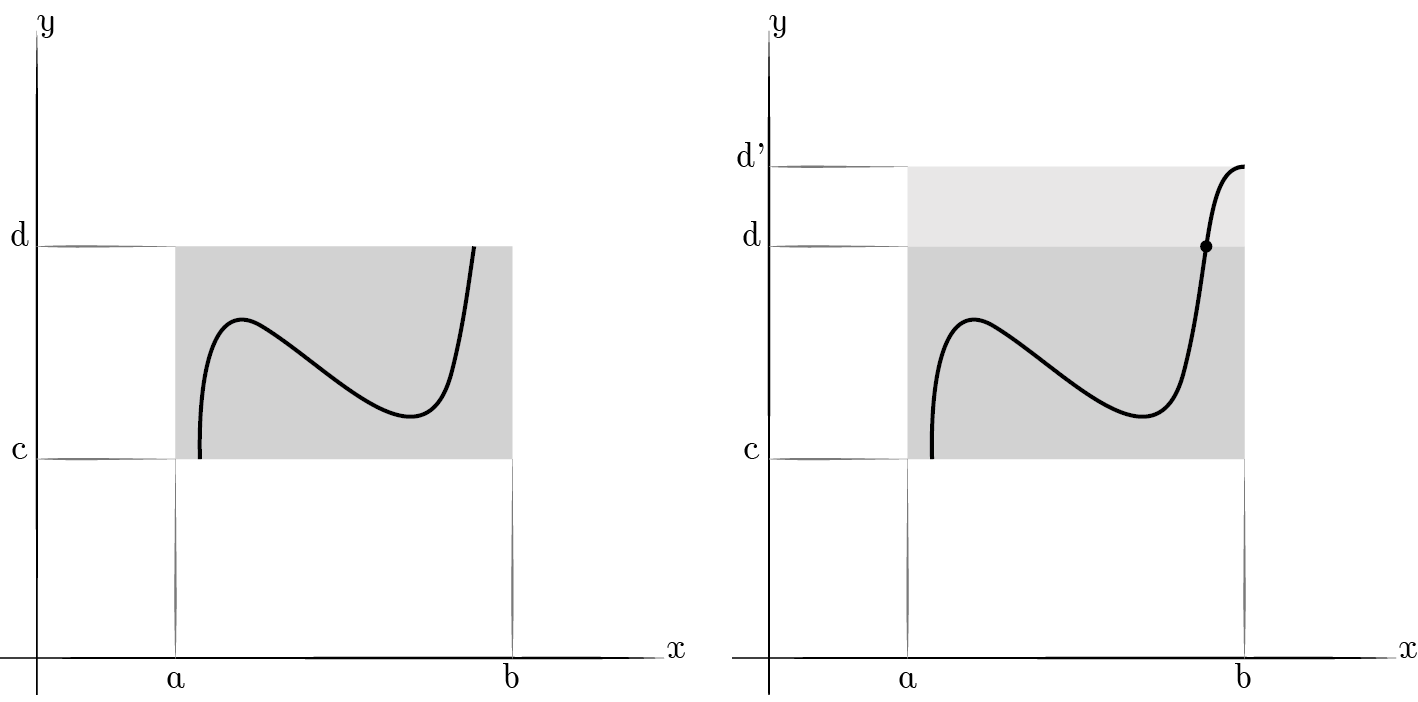
\includegraphics[width=0.7\textwidth]{1-prolongacion-solucion.png}}
        \end{center}
        Puede ocurrir que hayamos definido la función sobre un área más pequeña de lo necesario. En la imagen superior se representa esta casuística.\\
        En este caso, podemos prolongar la solución gracias a la unicidad, si existiera otra solución con $t\in[a,b]$ que estuviera definida en todo $[c, d']$, entonces debería coincidir con nuestra solución original por compartir el punto $(t, d)$. Podríamos preguntarnos  entonces si existe un intervalo cerrado máximo en el que existe nuestra solución.
        \item Acerca de las hipóstesis.\\
        No es necesario pedir que $f \in C^1$. Para la existencia sólo necesitamos que $f$ sea continua, y para la unicidad nos basta con que $f_x$ exista y sea continua. En el caso general veremos que podemos pedir incluso menos para la unicidad.
    \end{enumerate}
\end{obs}

\subsection{Regularidad de soluciones}
En ocasiones nos va a interesar saber como de buena es la función que resuelve nuestra EDO, entendiendo buena por cómo de suave es. Supongamos que nuestra ecuación diferencial es $x'(t) = f(t, x(t))$ definida en un intervalo, con $f:[a,b] \times [c,d] \subset \R^2 \longrightarrow \R$ continua y $x(t)$ derivable.\\
Entonces:
\begin{align*}
    x(t) \text{ derivable} &\implies x(t) \text{ continua}.\\
    \begin{cases}
        x(t) \text{ continua}\\
        f(t_1, t_2) \text{ continua}
    \end{cases} &\implies [\text{componiendo $f$ con $x(t)$ como $t_2=x(t)$})]\ f(t, x(t))\text{ es continua}\implies\\
     &\implies x'(t)\text{ es continua}\implies x(t) \in C^1
\end{align*}
Además, si $f(t_1, t_2) \in C^1$ entonces $f(t, x(t)) \in C^1$, pues:
$$
    \Dd{t}(f(t, x(t))) = f_t(t, x(t)) + f_x(t, x(t)) \cdot x'(t)
$$
De donde sabemos que tanto $f_t$ como $f_x$ son continuas pues $f(t_1, t_2) \in C^1$ y $x'(t)$ es continua como acabamos de ver. Y como $x''(t) = \Dd{t}(x'(t)) = \Dd{t}(f(t, x(t)))$ que es continua, entonces $x(t) \in C^2$.\\\\
Repitiendo este argumento, concluimos con que: $f(t_1,t_2) \in C^k \implies x(t) \in C^{k+1}$.

\section{Ecuaciones exactas}
Hasta ahora hemos visto como resolver ecuaciones de variables separables, homogéneas de grado 0 y lineales de orden I. Veamos un método más.\\\\
Supongamos que $\mbf{y}$ está definida implicitamente por $g(x, \mbf{y}) = cte$ con $g \in C^1$. Si derivamos $g(x, \mbf{y}) = cte)$ respecto de $x$ obtenemos:
$$
    g_x(x, y(x)) + g_y(x, y(x)) \cdot y'(x) = 0, \text{ es decir,}
$$
$y(x)$ se resuelve a partir de.
$$
    \mbf{y'} = -\frac{g_x(x,\mbf{y})}{g_y(x,\mbf{y})}
$$
\begin{obs}
    Podemos argumentar a la inversa. Si $y(x)$ verifica la EDO, entonces $g(x, y(x))$ es constante (en intervalos), pues $\Dd{x}(g(x, y(x))) = 0$
\end{obs}
Además, la notación habitual para este tipo de ecuaciones es:
$$
    \mbf{y'} = \dd{y}{x} = -\frac{g_x(x,\mbf{y})}{g_y(x,\mbf{y})} \implies g_x\d x + g_y \d y = 0
$$
Supongamos que tenemos una ecuación $y'(x) = \frac{M(x,y)}{N(x,y)}$, es decir, $M\d x + N \d y = 0$. Nos gustaría saber cuándo existe $g(x, \mbf{y}) : M = g_x,\ N = g_y$, ya que en ese caso es exacta y y su solución es $g(x, \mbf{y}) = C \mid C \text{constante}$ en forma implícita.
\begin{eg}[Ecuación exacta simple]
    Sea $\mbf{y'} = \frac{-\mbf{y}}{x}$, es decir, $\mbf{y}\d x + x \d y = 0$ es una ecuación exacta.\\
    De hecho la $g$ necesaria es $g(x,\mbf{y}) = xy$ pues $g_x = \mbf{y}$ y $g_y = x$. Y por tanto, la solucion general es:
    $$
        x\mbf{y} = C \implies y(x) = \frac{C}{x}
    $$
    De hecho, esta ecuación es de los tres tipos que hemos visto.
\end{eg}
\begin{pro}[Condición necesaria de ecuación exacta]
    $$
        \mathcal{EC} \equiv M\d x + N\d y \text{ es exacta y }g(x, \mbf{y}) \in C^2 \implies M_y = N_x
    $$
\end{pro}
\begin{proof}
    Si $\mathcal{EC}$ es exacta, entonces $\exists g : M = g_x,\ N = g_y$. Como $g \in C^2$, sabemos que $g_{xy} = g_{yx}$, entonces:
    $$
        \begin{cases}
            g_{xy} = (g_x)_y = M_y\\
            g_{yx} = (g_y)_x = N_x
        \end{cases} \implies M_y = N_x
    $$
\end{proof}
\begin{obs}
    Sabemos que una ecuación es exacta cuando $(M, N) = \Nabla g$, sea $\gamma$ cualquier curva tal que $\gamma : [a,b]\subset\R \longrightarrow \R^2$ en $\R^2$. Entonces:
    $$
        \int_\gamma M\d x + N\d y = g(\gamma(b)) - g(\gamma(a))
    $$
    Es claro que si la curva es cerrada, $\gamma(a)=\gamma(b)$ y la integral es nula.
\end{obs}

\begin{eg}[Ecuación exacta]
    Sea $\mathcal{(EC)} \equiv (\mbf{y}+x^3) dx + (x+\mbf{y}^3) dy = 0$ es facil ver que cumple la condición de $M_x = N_y$.\\
    Nos gustaría hallar cual sería nuestra $g$ a partir de que $g_x=M$ y $g_y=N$. Sabemos que $g_x = M = y + x^3$.
    Si integramos en $x$ (suponiendo $\mbf{y}$ constante):
    $$
    g(x,\mbf{y} = yx + x^4/4 + C(y) \text{para C una constante vista desde $x$}.
    $$
    Además,
    \begin{gather*}
        x+\mbf{y}^3 = N = g_y = x + c'(\mbf{y}) \implies c'(\mbf{y}) = \mbf{y}^3\\
        c'(\mbf{y}) = \mbf{y}^3 \implies c(\mbf{y}) = \frac{\mbf{y}^4}{4} + cte.
    \end{gather*}

    Por lo que tenemos: $g(x,\mbf{y}) = x\mbf{y} + \frac{x^4+\mbf{y}^4}{4}$. Es decir, las soluciones de $\mathcal{(EC)}$ vienen dadas por $xy + \frac{x^4+y^4}{4} = C \text{($C$ constante)}$.\\

    Por ejemplo, una solución particular para C=1 es:

    $$xy + \frac{x^4+y^4}{4} = 1, \text{ que es la curva roja en la imagen siguiente.}$$
    \begin{center}
        \raisebox{\dimexpr \topskip-\height}{
      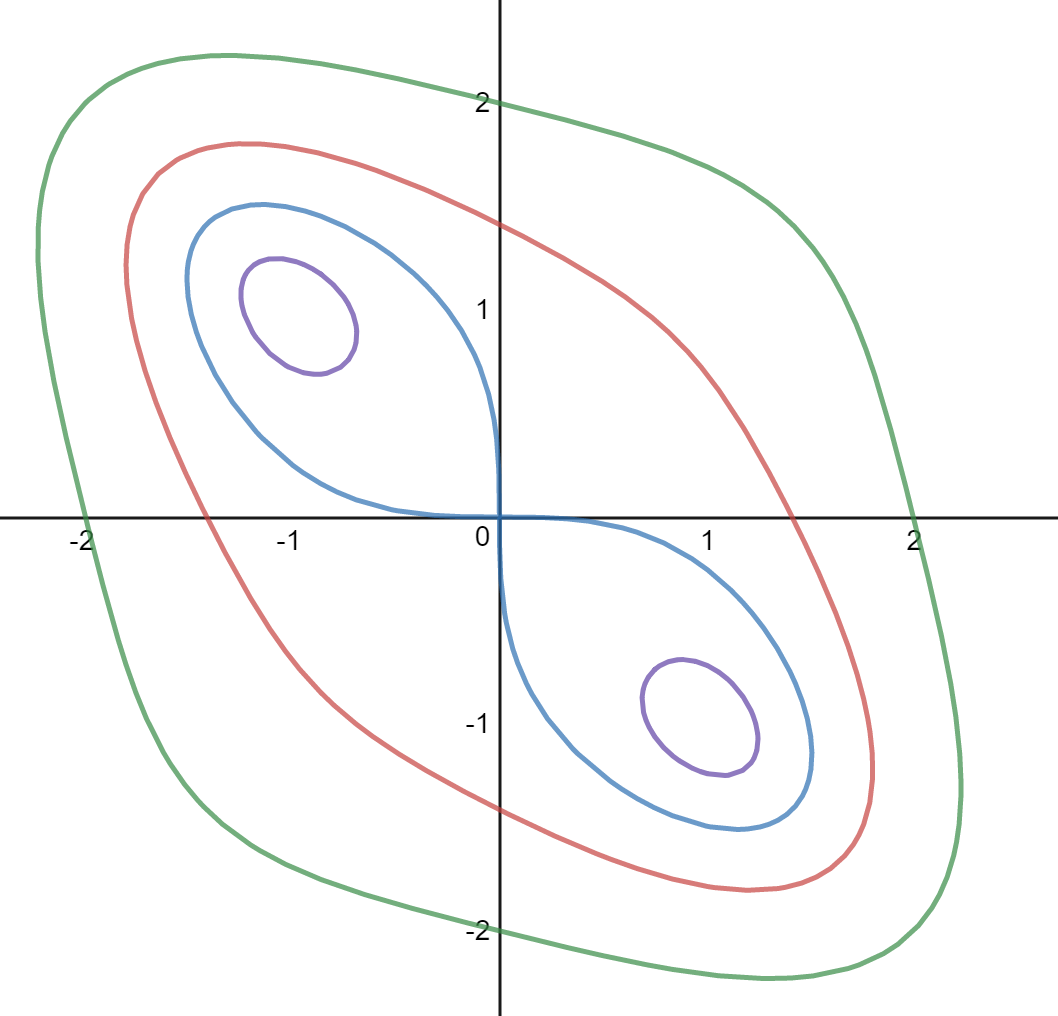
\includegraphics[width=0.5\textwidth]{1-ecuacion-exacta.png}}
    \end{center}
\end{eg}

Queremos ahora analizar la condición necesaria y suficiente que nos asegure que podamos realizar el procedimiento del ejemplo. Haremos uso de la siguiente proposición.
\begin{pro}
Sea $\Omega\subset\R^2$ un abierto simplemente conexo. Sean $M, N : \Omega \to \R\text{ con } M,N \in C^1$, entonces:
$$
\exists g : \Omega \to \R \text{ con } g \in C^2 \text{ tal que } M = \left.g_x\right|_\Omega, \left.N=g_y\right|_\Omega \iff \left.M_y\right|_\Omega = \left.N_x\right|_\Omega.
    $$
\end{pro}
La demostración se deja al lector.\\\\
A modo de recordatorio vamos a dar una definición de \textit{abierto simplemente conexo}.
\begin{dfn}
    Sea $\Omega \subset \R^2$ un abierto acotado.\\
    Decimos que $\Omega$ es \textbf{simplemente conexo} $\iff$ $\Omega^C = \R^2\Omega$ es conexo.
\end{dfn}

\section{Factores integrantes}
Sea de nuevo $\mathcal{(EC)}_1 = M \d x + N\d y = 0$, pero supongamos ahora que no se cumple la condición $M_x = N_y$ necesaria para encontrar una ecuación exacta. Nos preguntamos si podemos encontrar un $\mu(x, \mbf{y})$ no trivial de forma que teniendo la ecuación $\mathcal{(EC)}_2 = \mu(x, \mbf{y}) M \d x + \mu(x, \mbf{y}) N\d y = 0$ se cumpla:
\begin{equation}\label{eq:factor-integrante}
    (\mu M)_y = (\mu N)_x
\end{equation}
Llamamos a $\mu$ factor integrante de $\mathcal{(EC)}_1$. Veremos que siempre existe pero que es dificil de encontrar.\\
Calculando \ref{eq:factor-integrante}, obtenemos:
\begin{gather*}
    M \frac{\partial \mu}{\partial y} - N \frac{\partial \mu}{\partial x} + (M_y - N_x) \mu = 0\\
    \left(M \frac{\partial}{\partial y} - N \frac{\partial}{\partial x}\right)\mu + (M_y - N_x) \mu = 0
\end{gather*}
de donde tendremos que calcular $\mu$. Como suele resultar difícil, habitualmente se intenta que $\mu$ solo dependa de una de las dos variables, es decir, $\mu=\mu(y)$ o $\mu=\mu(x)$.\\\\

%%%%%%%%%%%%%%%%%%%%%%%%%%%%%%%%%%%%%%%%%%%%%%%%%%%%%%%%%%%%%%%% Clase del 11/02
Veamos un ejemplo de ecuacion de factores integrantes
\begin{eg}[Factores integrantes]
    Sea $x\mbf{y}\ \d x + \mb{y}^2 \d y = 0$, esta claro que $M = x\mbf{y}$, $N = \mbf{y}^2$. Para ver si puede ser una ecuación exacta evaluamos si cumple la condición necesaria $M_y = N_x$, sin embargo las derivadas cruzadas son $M_y=x$ y $N_x = 0$ y por tanto no puede ser ecuación exacta.\\\\
    Nos preguntamos entonces por cual es su factor integrante. Para encontrarlo vamos a intentar que $\mu$ dependa solo de una variable (o de una combinación lineal, i.e $z = x+y$).\\
    \begin{enumerate}
        \item \texttt{Intentamos que $\mu$ dependa de $x$.}\\\\
            Transformamos nuestra ecuación en: $(\mathcal{EC})\equiv \mu M\ \d x + \mu N\ \d y = 0$. Es decir, tenemos:
            $$
                \mu(x)\ x\mbf{y}\  \d x + \mu(x)\ \mbf{y}^2\ \d y = 0, \text{entonces hallamos las nuevas $M_y$ y $N_x$ para hallar $\mu$}
            $$
            como se tiene que cumplir que $M_y = N_x$
            $$
                M_y = \mu(x)\ x = \mu'(x)\ \mbf{y}^2 = N_x \implies \frac{\mu'(x)}{\mu(x)} = \frac{x}{\mbf{y}}
            $$
            y es claro que no tiene solución, pues la parte de la izquierda no depende de y.
        \item \texttt{Intentamos que $\mu$ dependa de $\mbf{y}$.}\\\\
        Repitiendo el mismo procedimiento, hallamos las nuevas $M_y$ y $N_x$ para hallar $\mu$ que cumple la condición necesaria. Obtenemos:\\\\
        $$
            \frac{\mu'(y)}{\mu(y)} = \frac{-1}{y} \implies (log |\mu|) = -log |y| \implies \mu(y) = \frac{1}{y} \text{ es solución}.
        $$
        Es decir, $(\mathcal{EC}) \equiv x\ \d x + \mbf{y}\ \d y = 0$. Podemos resolverla por separación de variables y su solución es:
        $$
            \frac{x^2+\mbf{y}^2}{2} = C \implies x^2+\mbf{y}^2 = C
        $$
    \end{enumerate}
\end{eg}

\begin{obs}
    Sea la ecuación lineal de primer orden $\mbf{y}' = a(x) \cdot \mbf{y} + b(x)$.\\
    Con $A(x) : A'(x) = a(x)$ $(e^{A(x)})$. %%TODO: Completar
    Entonces $e^{-A(x)}$ es un factor integrante de $y'(x) = a(x) \cdot y(x) + b(x)$.
\end{obs}

\begin{eg}[Análisis de cotas en una ecuación diferencial]
Vamos a hacer un aparte para retomar el ejemplo \ref{eg:campo-pendientes}. Teníamos que $(\mathcal{EC}1) \equiv \mbf{x}' = t^2 + \mbf{x}^2 = f(t, \mbf{x})$ y llegábamos a la conclusión a través de trazar su campo de pendientes de que $x(t) \uparrow \infty$, pero no sabíamos si lo hacía de forma asintótica o lo alcanza cuando $t \to \infty$, aunque el campo parecía indicar que lo hacía de forma asintótica en $t=1$ o antes. Vamos a tratarla de forma analítica comparándola con otra ecuación que se asemeja y que ya conocemos.\\\\
Sabemos que $|f_x| < L$ no se cumple, pues $2x \to \infty$ si $x \to \infty$ y no podemos aplicar el teorema de existencia y unicidad global.\\
Vamos a comparar la solución de $(\mathcal{EC}1)$ donde exista con la de:
$$
    (\mathcal{EC}2)\equiv
    \begin{cases}
        \mbf{x}' = \mbf{x}^2\\
        x(0) = 1
    \end{cases}
$$
Sean $u(t)$ la solución de $(\mathcal{EC}1)$ y $v(t)$ la solución de $(\mathcal{EC}2)$. A primera vista en $t=0$ ambas tienen la misma pendiente pues $f(0,1) = 1$.
Sabemos tambien que $u(t)$ crece más rapido que $v(t)$ por que en el momento en que $t \neq 0$, crecerá más rápido (pues $t^2 + x(t^2) \geq x(t^2)$). Cualitativamente podemos afirmar que $u(t)$ "va por encima" de $v(t)$. Nos gustaría hacer una comparativa cuantitativa de ambas.\\\\
Para ello, consideramos $z(t) = u(t) - v(t)$. Ahora, calculamos $z'(t)$:
$$
    z'(t) =  u'(t) - v'(t) = t^2+u^2-v^2 = t^2 + (u - v)\cdot(u + v) = t^2 + \mbf{z}\cdot(u + v).
$$
En este caso no conocemos explícitamente $(u(t)+v(t))$, pero podemos afirmar que como $(u(t),v(t))$ son crecientes $\forall t\geq0$ y para $t=0$ valen 1, entonces $(u + v) \geq 2$. Por tanto,
$$
    \mbf{z}' \geq 2\mbf{z} + t^2 \implies \mbf{z}' - 2\mbf{z}\geq t^2.
$$
Sea $w(t) = e^{-2t}\cdot z(t)$, entonces $\mbf{w}' = e^{-2t}(\mbf{z}'-2\mbf{z}) \geq e^{-2t}t^2 \geq t^2$. Entonces $\mbf{w}' \geq e^{-2t}t^2$ y además $w(0) = z(0) = 1 - 1 = 0$. A partir de esto tenemos:
$$ %%TODO: Preguntar por esta definición de w(t)
    w(t) = w(0) + \int_0^t w'(s) \d s \geq \int_0^t s^2 e^{-2s} \d s = \left.e^{-2s} \cdot \frac{2s^2 + 2s + 1}{4}\right|_0^t
$$
es decir,
$$
    w(t) \geq \frac{1}{4} - e^{-2t} \frac{2t^2 + 2t + 1}{4} \text{, y como } w(t) = e^{-2t} z(t) \text{ entonces,}
$$
$$
    z(t) \geq \frac{e^{2t} - (2t^2 + 2t + 1) }{4} \implies u(t) - v(t) \geq \frac{e^{2t} - (2t^2 + 2t + 1) }{4} \implies u(t) \geq v(t) + \frac{e^{2t} - (2t^2 + 2t + 1) }{4}
$$
Como vimos en \ref{eg:no-solution}, $v(t) = \frac{1}{1-t}$ y por tanto $v \to \infty$ cuando $t \to 1$. Y ya que $u(t) \geq v(t) + \frac{e^{2t} - (1 + 2t + 2t^2)}{4}$, $u \to \infty$ antes de $t = 1$.
\end{eg}
\begin{th_ex} %TODO: Que cojones es esto
    Encontrar otra ecuacion que sea sencilla de resolver para $u(t) \geq x$.
\end{th_ex}

%%%%%%%%%%%%%%%%%%%%%%%%%%%%%%%%%%%%%%%%%%%%%%%%%%%%%%%%%%%%%%%% Clase del 12/02

\section{Ecuaciones de orden II}
Hasta ahora hemos estudiado distintas ecuaciones de orden I. Vamos a ver un nuevo tipo de ecuaciones que involucra la segunda derivada y hay diversos ejemplos en el estudio de la Física.

\begin{dfn}[Ecuaciones de orden II]
    Sea $\mbf{x} = f(t)$, una \textbf{ecuación diferencial de segundo orden} es una ecuación de la forma: $\mbf{x}'' = F(t, \mbf{x}, \mbf{x}')$
\end{dfn}

\begin{obs}
    La ecuación $\mbf{x}'' = 5\mbf{x}'$ es de orden 2 sólo formalmente, ya que se resuelve como una de primer orden. Con $y(t) = 5\mbf{y}, \mbf{y}' = 5\mbf{y} \implies y(t) = ce^{5t} \implies x(t) = \int C e^{5t} = a + b e^5t$. Sin embargo tenemos dos parametros, para determinarlos necesitamos añadir dos condiciones.El PVI entonces sería del tipo:
    $$
        \begin{cases}
            \mbf{x}'' = 5\mbf{x}'\\
            x(0) = 1\\
            x'(0) = 0
        \end{cases}
    $$
    Con esto hallaríamos $a+b = 1$, $b=0$.\\\\
    Sin embargo, podemos tener otro tipo de condiciones que no serían un PVI, por ejemplo, dar dos condiciones para x(t) y ninguna para x'(t). Estas no tienen aseguradas existencia y unicidad y lo veremos más adelante.
\end{obs}

Como fuente de ejemplos para esta sección utilizaremos la segunda ley de Newton $F = m\cdot a$.

\begin{eg}[Muelles]\label{eg:muelle}
    %%TODO: Incluir dibujo del muelle.
      \begin{center}
        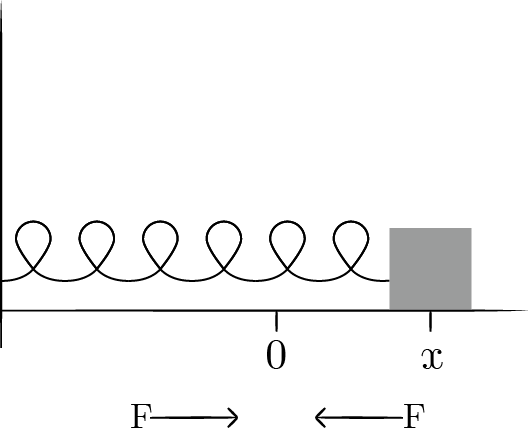
\includegraphics[height=0.1\textheight]{1-muelle.png}
      \end{center}
        Consideramos que $x=0$ corresponde a la situación de equilibrio, es decir totalmente parado. Además vamos a suponer que:
        \begin{itemize}
            \item no hay fricción con la superficie ni con el aire.
            \item tenemos movimientos oscilatorios desde la situación de equilibrio.
            \item la masa es puntual.
        \end{itemize}
        La fuerza por tanto se expresa como $F = -k x$, donde $k$ es la constante del muelle y es negativa por que va en sentido contrario al vector posición con origen en $x=0$.\\\\
        La ecuación diferencial de este modelo es:
        $$
            m\mbf{x}'' = -k \mbf{x} \implies \mbf{x}'' = -\frac{k}{m}\cdot \mbf{x}
        $$
    Consideramos que $x=0$ corresponde a la situación de equilibrio, es decir totalmente parado. Además vamos a suponer que:
    \begin{itemize}
        \item no hay fricción con la superficie ni con el aire.
        \item tenemos movimientos oscilatorios desde la situación de equilibrio.
        \item la masa es puntual.
    \end{itemize}
    La fuerza por tanto se expresa como $F = -k x$, donde $k$ es la constante del muelle y es negativa por que va en sentido contrario al vector posición con origen en $x=0$.\\\\
    La ecuación diferencial de este modelo es:
    $$
        m\mbf{x}'' = -k \mbf{x} \implies \mbf{x}'' = -\frac{k}{m}\cdot \mbf{x}
    $$
    Vamos a hallar sus soluciones. Definimos $y(t) = x(\alpha t)$ (para \textit{esconder} el parametro $\frac{k}{m}$), vamos a ver cual es este $\alpha$:
    $$
    \mbf{y}'' = \alpha^2\cdot \mbf{x}''(\alpha t) = a^2\left(-\frac{k}{m}\cdot x(\alpha t)\right) = -\frac{k}{m} \alpha ^2\cdot y(t)
    $$
    Eligiendo $\alpha = \sqrt{\frac{m}{k}}$ tenemos $\mbf{y}'' = -\mbf{y}$. Vemos fácilmente que:\\\\
    \begin{enumerate}
        \item $\sin (t)$ y $\cos(t)$ son soluciones.
        \item $\mbf{y}'' = \mbf{y}$ es lineal.\\\\
        Es decir, si $y_1(t), y_2(t)$ son solución, entonces:
        $$
            \alpha_1 \mbf{y}_1 + \alpha_2 \mbf{y}_2 \text{ es solución } \forall \alpha_1, \alpha_2 \in \R
        $$
        Entonces con $\mbf{y}_1 = \sin$, $\mbf{y}_2 = \cos$ sabemos que:
        $$
            \alpha_1\sin(t) + \alpha_2\cos(t) \text{ es solución.}
        $$
        A priori no sabemos si estas son todas las soluciones. Podemos asegurar que sí con el teorema \ref{thm:exist-unic-ii} que se enuncia tras este ejemplo.\\\\
        Dados cualquier $y_0$, $y_1$ entonces:
        $$
            \exist \alpha, \beta : \mbf{y}_{\alpha, \beta} = \alpha \sin (t) + \beta \cos (t)
        $$
        que cumplen:
        $$
            \beta = y_{\alpha, \beta} (0) = y_0.\text{         } \alpha = y_{\alpha, \beta}'(0) = y_1.
        $$
        es decir, $\alpha, \beta$ forman el vector $(\alpha$ $\beta)$ = $(y_1$ $y_0)$. Por tanto, en el momento en que sepamos el valor $y(0)$, $y'(0)$ lo hemos resuelto pues $y(t) = y(0) \cos (t) + y'(0) \sin (t)$.
    \end{enumerate}
\end{eg}

\begin{thm}[Existencia y unicidad para ecuaciones lineales de orden II]\label{thm:exist-unic-ii}
    Sean: \\$(\mathcal{EC}) \equiv \mbf{x}'' + p(t)\mbf{x}' + q(t) \mbf{x} = r(t)$ con $p, q, r: [a, b] \subset \R \to \R$ continuas y $t_0 \in [a, b]$, $x_0,\ x_1 \in R$ entonces existe una solución y es única al PVI:
    $$
        \begin{cases}
            \mbf{x}'' + p(t)\mbf{x}' + q(t)\mbf{x} = r(t),\ \forall t \in [a, b].\\
            x(t_0) = x_0\\
            x'(t_1) = x_1\\
        \end{cases}
    $$
\end{thm}
La demostración de nuevo se deja para el caso general.\\\\
Vamos a enunciar ciertas propiedades.
\begin{enumerate}
    \item Es lineal, el conjunto de soluciones es un espacio vectorial.
    $$
        \text{Sean } \mbf{x}_1, \mbf{x}_2 \text{ soluciones, } \alpha_1, \alpha_2 \in \R \implies \alpha_1 x_1(t) + \alpha_2 x_2(t) \text{ es solución.}
    $$
    \item Ese espacio vectorial tiene dimensión 2.
\end{enumerate}
\begin{proof} (\textit{A las propiedades})\\
    \begin{enumerate}
        \item Se demuestra como en el ejemplo.
        \item Sea $x_1$ la solución del PVI:
        $$
        \begin{cases}
            \mbf{x}'' + p(t) \mbf{x}' + q(t) \mbf{x} = 0\\
            x(a) = 1\\
            x'(a) = 0
        \end{cases}
        $$
        y sea $x_2$ la solución del PVI:
        $$
        \begin{cases}
            \mbf{x}'' + p(t) \mbf{x}' + q(t) \mbf{x} = 0\\
            x(a) = 0\\
            x'(a) = 1
        \end{cases}
        $$
        Por existencia y unicidad, $\mbf{x}_1, \mbf{x}_2$ existen en $[a,b]$. Además, ninguna es un múltiplo de la otra, es decir, son linealmente independientes pues:
        \begin{itemize}
            \item Cualquier $\mbf{x} = \alpha \mbf{x}_1$ cumple $x'(a) = 0$ pero $x_2'(a) \neq 0$.
            \item Cualquier $\mbf{x} = \beta \mbf{x}_2$ cumple $x(a) = 0$ pero $x_1(a) \neq 0$.
        \end{itemize}
        Por tanto, la dimensión del espacio de soluciones es al menos 2. Para ver que es justo dos se sigue:\\\\
        Dada cualquier solución x(t) de la ecuación
        $$
            x(t) = x(a) \cdot x_1(t) + x'(a) \cdot x_2(t)
        $$ %%TODO: Clarificar.
        por unicidad, el término de la derecha es solución con:
        $$
            \begin{cases}
                \text{ valor en a igual a $x(a)$}\\
                \text{ derivada en a igual a $x'(a)$}
            \end{cases}
        $$
    \end{enumerate}
\end{proof}

\begin{obs}
    Como vimos en el ejemplo \ref{eg:muelle}, para resolver $\mbf{x}'' + p(t) \mbf{x}' + q(t) \mbf{x} = 0$ basta encontrar dos soluciones linealmente independientes.
\end{obs}

\begin{eg}[Ecuaciones de orden II como sistemas]
    Cosideramos $(\mathcal{EC} \equiv f(t, \mbf{x}, \mbf{x}'))$. Sea $\mbf{y} = \mbf{x'}$, entonces podemos resolverla resolviendo un sistema de ecuaciones. Para ello consideraremos el vector $X(t) = \left[\begin{smallmatrix} x(t) \\ y(t) \end{smallmatrix}\right]$. Si derivamos:
    $$
        X'(t) = \left[\begin{matrix} x'(t) \\ y'(t) \end{matrix}\right] = \left[\begin{matrix} y \\ f(t, x, x') \end{matrix}\right]= \left[\begin{matrix} y \\ f(t, x, y) \end{matrix}\right] = F(t, X)
    $$
    Con lo que llegamos a la expresión:
    $$
        X'(t) = F(t, X) \text{ que representa un sistema de ecuaciones}
    $$
    %%TODO: Clarificar

\end{eg}

%%%%%%%%%%%%%%%%%%%%%%%%%%%%%%%%%%%%%%%%%%%%%%%%%%%%%%%%%%%%%%%% Clase del 13/02
